% !TeX program = pdflatex
% Отчёт по заданию 3 «Снижение размерности и кластеризация. Общие режимы
% гидравлического испытательного стенда» (вариант 13), ГОСТ 7.32-2017.
% Все числа вставляются макросами из tables/macros.tex (см. src/modeling.py);
% ручное редактирование чисел не используется.
\documentclass[14pt,a4paper]{extarticle}

\usepackage[T2A]{fontenc}
\usepackage[utf8]{inputenc}
\usepackage[russian]{babel}
\usepackage{tempora}                % Times-подобный текстовый шрифт
\usepackage{amsmath}
\usepackage{graphicx}
\usepackage{booktabs}
\usepackage{array}
\usepackage{float}
\usepackage{setspace}
\usepackage[a4paper,top=20mm,bottom=20mm,left=30mm,right=15mm]{geometry}
\usepackage{caption}
\usepackage{titlesec}
\usepackage{lastpage}
\usepackage[unicode,hidelinks]{hyperref}

% --- Оформление по ГОСТ 7.32-2017 -----------------------------------------
\onehalfspacing
\setlength{\parindent}{12.5mm}
\setlength{\parskip}{0pt}
\setlength{\emergencystretch}{2em}
\setcounter{tocdepth}{2}

\providecommand{\textminus}{\ensuremath{-}}

% «Рисунок N --- Название» под рисунком, «Таблица N --- Название» над таблицей
\DeclareCaptionLabelSeparator{gostdash}{ --- }
\captionsetup[table]{labelsep=gostdash,justification=raggedright,
  singlelinecheck=false,position=above,skip=6pt}
\captionsetup[figure]{labelsep=gostdash,justification=centering,
  singlelinecheck=false,position=below,skip=6pt}
\addto\captionsrussian{%
  \renewcommand{\figurename}{Рисунок}%
  \renewcommand{\tablename}{Таблица}%
}

% Заголовки разделов: с абзацного отступа, полужирные
\titleformat{\section}{\bfseries\raggedright}{\thesection}{0.6em}{}
\titleformat{\subsection}{\bfseries\raggedright}{\thesubsection}{0.6em}{}
\titlespacing*{\section}{\parindent}{14pt}{10pt}
\titlespacing*{\subsection}{\parindent}{12pt}{8pt}

% Список источников: «1.» в перечне, без собственного заголовка
\makeatletter
\renewcommand{\@biblabel}[1]{#1.}
\renewenvironment{thebibliography}[1]
     {\list{\@biblabel{\@arabic\c@enumiv}}%
           {\settowidth\labelwidth{\@biblabel{#1}}%
            \leftmargin\labelwidth
            \advance\leftmargin\labelsep
            \usecounter{enumiv}%
            \let\p@enumiv\@empty
            \renewcommand\theenumiv{\@arabic\c@enumiv}}%
      \sloppy
      \clubpenalty\@clubpenalty
      \widowpenalty4000%
      \sfcode`\.\@m}
     {\def\@noitemerr
       {\@latex@warning{Empty `thebibliography' environment}}%
      \endlist}
\makeatother
\addto\captionsrussian{%
  \renewcommand{\refname}{СПИСОК ИСПОЛЬЗОВАННЫХ ИСТОЧНИКОВ}%
}

% Содержание: заголовок по центру, список без полуторного интервала
\makeatletter
\renewcommand\tableofcontents{%
  \clearpage
  \begin{spacing}{1.0}%
  \begin{center}\bfseries СОДЕРЖАНИЕ\end{center}%
  \@starttoc{toc}%
  \end{spacing}%
}
\makeatother

% Структурный элемент: с нового листа, прописными, по центру
\newcommand{\struct}[1]{%
  \clearpage
  \begin{center}\bfseries #1\end{center}%
  \addcontentsline{toc}{section}{#1}%
}

% Автоматически сгенерировано src/modeling.py; не редактировать.

\newcommand{\NSrc}{11}
\newcommand{\NApp}{2}
\newcommand{\NFig}{14}
\newcommand{\NTab}{14}
\newcommand{\DataCycles}{2205}
\newcommand{\DataChannels}{7}
\newcommand{\DataFeaturesAll}{28}
\newcommand{\DataFeaturesUsed}{25}
\newcommand{\DataConstant}{2}
\newcommand{\DataNearConstant}{3}
\newcommand{\DataConstantList}{PS2\_min, PS3\_min}
\newcommand{\DataNearConstantList}{PS2\_min, PS3\_min, FS1\_min}
\newcommand{\DataMissing}{0}
\newcommand{\DataDuplicates}{0}
\newcommand{\DataOutliers}{2372}
\newcommand{\DataOutlierShare}{3,84}
\newcommand{\DataTrain}{1544}
\newcommand{\DataTest}{661}
\newcommand{\DataTrainFirst}{1}
\newcommand{\DataTrainLast}{1544}
\newcommand{\DataTestFirst}{1545}
\newcommand{\DataTestLast}{2205}
\newcommand{\BlockTrain}{1505}
\newcommand{\BlockTest}{700}
\newcommand{\BlockSize}{50}
\newcommand{\ValvePerLevel}{360}
\newcommand{\ValveOptimal}{1125}
\newcommand{\CoolerPerLevel}{732}
\newcommand{\StableOne}{756}
\newcommand{\CoolerLast}{741}
\newcommand{\PcaEvrOne}{0,5442}
\newcommand{\PcaEvrTwo}{0,2373}
\newcommand{\PcaEvrThree}{0,0559}
\newcommand{\PcaEvrFour}{0,0532}
\newcommand{\PcaEvrFive}{0,0334}
\newcommand{\PcaEvrSix}{0,0218}
\newcommand{\PcaCumTwo}{0,7815}
\newcommand{\PcaCumThree}{0,8374}
\newcommand{\PcaCumFour}{0,8906}
\newcommand{\PcaCumFive}{0,9240}
\newcommand{\PcaCumSix}{0,9458}
\newcommand{\PcaCumTen}{0,9938}
\newcommand{\PcaCentEvrOne}{0,6508}
\newcommand{\PcaCentCumTwo}{0,9927}
\newcommand{\PcaCentCumFour}{0,9994}
\newcommand{\PcaRmseStdTwo}{5,518}
\newcommand{\PcaRelStdTwo}{0,530}
\newcommand{\PcaRelStdFour}{0,414}
\newcommand{\PcaRelStdSix}{0,384}
\newcommand{\PcaRelStdTen}{0,162}
\newcommand{\PcaRmseCentTwo}{1,720}
\newcommand{\PcaRelCentTwo}{0,572}
\newcommand{\PcaRelCentTen}{0,405}
\newcommand{\PcaRelStdTwoBlocked}{0,734}
\newcommand{\PcaRelCentTwoBlocked}{0,772}
\newcommand{\PcaClusterShare}{0,8906}
\newcommand{\PcaPcOneCorr}{\textminus{}0,774}
\newcommand{\FaLlTrainTwo}{\textminus{}3,79}
\newcommand{\FaLlTestTwo}{\textminus{}11,09}
\newcommand{\FaLlBlockedTwo}{\textminus{}22,65}
\newcommand{\FaNoiseTwo}{0,238}
\newcommand{\FaCommTwo}{0,762}
\newcommand{\FaIterTwo}{286}
\newcommand{\FaLlTrainThree}{\textminus{}0,22}
\newcommand{\FaLlTestThree}{\textminus{}13,08}
\newcommand{\FaLlBlockedThree}{\textminus{}21,48}
\newcommand{\FaNoiseThree}{0,224}
\newcommand{\FaCommThree}{0,776}
\newcommand{\FaIterThree}{443}
\newcommand{\FaLlTrainFive}{5,75}
\newcommand{\FaLlTestFive}{\textminus{}11,89}
\newcommand{\FaLlBlockedFive}{\textminus{}16,39}
\newcommand{\FaNoiseFive}{0,153}
\newcommand{\FaCommFive}{0,847}
\newcommand{\FaIterFive}{482}
\newcommand{\FaBestK}{2}
\newcommand{\ClustN}{1200}
\newcommand{\ClustShareOfAll}{54,4}
\newcommand{\ClustPcs}{4}
\newcommand{\ClustShare}{0,8906}
\newcommand{\ClustSharePct}{89,1}
\newcommand{\RuleStab}{0,90}
\newcommand{\RuleShare}{5}
\newcommand{\RuleSil}{95}
\newcommand{\KmK}{3}
\newcommand{\KmSil}{0,588}
\newcommand{\KmDb}{0,634}
\newcommand{\KmStab}{1,00}
\newcommand{\KmAriCooler}{0,582}
\newcommand{\KmAriValve}{0,038}
\newcommand{\KmAriAccum}{0,039}
\newcommand{\KmAriPump}{0,096}
\newcommand{\KmAriAg}{0,980}
\newcommand{\KmAriDb}{0,705}
\newcommand{\KmSizeOne}{127}
\newcommand{\KmSizeTwo}{675}
\newcommand{\KmSizeThree}{398}
\newcommand{\KmCycleOne}{212--702}
\newcommand{\KmCycleTwo}{8--1467}
\newcommand{\KmCycleThree}{1472--2205}
\newcommand{\KmStableOne}{1,6}
\newcommand{\KmStableTwo}{40,9}
\newcommand{\KmStableThree}{31,9}
\newcommand{\WardSil}{0,578}
\newcommand{\WardDb}{0,604}
\newcommand{\WardStab}{0,99}
\newcommand{\WardAriCooler}{0,577}
\newcommand{\WardAriValve}{0,035}
\newcommand{\WardAriAccum}{0,035}
\newcommand{\WardAriPump}{0,104}
\newcommand{\KFourSil}{0,582}
\newcommand{\KFourAriCooler}{0,879}
\newcommand{\KFiveSil}{0,598}
\newcommand{\KSixSil}{0,617}
\newcommand{\KSixSizeMin}{12}
\newcommand{\DbEps}{0,6}
\newcommand{\DbEpsRule}{0,501}
\newcommand{\DbMinSamples}{10}
\newcommand{\DbNClusters}{4}
\newcommand{\DbNoise}{5,0}
\newcommand{\DbSil}{0,635}
\newcommand{\DbDb}{0,618}
\newcommand{\DbAriCooler}{0,906}
\newcommand{\DbAriValve}{0,013}
\newcommand{\DbAriAccum}{0,096}
\newcommand{\DbSizeOne}{224}
\newcommand{\DbSizeTwo}{114}
\newcommand{\DbSizeThree}{405}
\newcommand{\DbSizeFour}{397}
\newcommand{\DbMsFiveNoise}{3,2}
\newcommand{\DbMsTwentyNoise}{6,5}
\newcommand{\KmSilTwo}{0,528}
\newcommand{\KFiveSizeMin}{11}
\newcommand{\DbStableOne}{50,4}
\newcommand{\DbCycleOne}{25--732}
\newcommand{\DbStableTwo}{0,9}
\newcommand{\DbCycleTwo}{212--691}
\newcommand{\DbStableThree}{34,3}
\newcommand{\DbCycleThree}{740--1465}
\newcommand{\DbStableFour}{32,0}
\newcommand{\DbCycleFour}{1472--2205}
\newcommand{\WardSizeOne}{118}
\newcommand{\WardSizeTwo}{684}
\newcommand{\WardSizeThree}{398}
\newcommand{\DataHighPressN}{240}
\newcommand{\DataHighPressShare}{10,9}
\newcommand{\DataHighPressRange}{212--702}
\newcommand{\DataHighPressSub}{127}
\newcommand{\HighFlagPsOne}{173,0}
\newcommand{\HighRestPsOne}{159,0}
\newcommand{\HighFlagFsOne}{3,28}
\newcommand{\HighRestFsOne}{6,55}
\newcommand{\HighFlagTsOne}{56,8}
\newcommand{\HighRestTsOne}{44,0}
\newcommand{\HighFlagPsThree}{1,10}
\newcommand{\HighRestPsThree}{1,83}
\newcommand{\HighFlagEpsOne}{2623}
\newcommand{\HighRestEpsOne}{2480}
\newcommand{\KmGTwoCoolerThree}{266}
\newcommand{\KmGTwoCoolerTwenty}{407}
\newcommand{\KmGTwoCoolerHundred}{2}
\newcommand{\KmGOneCoolerThree}{127}
\newcommand{\KmGThreeCoolerHundred}{398}
\newcommand{\DriftTsOneEarly}{55,0}
\newcommand{\DriftVsOneEarly}{0,680}
\newcommand{\DriftEpsOneEarly}{2474}
\newcommand{\DriftPsOneEarly}{162,1}
\newcommand{\DriftPcOneEarly}{2,87}
\newcommand{\DriftTsOneMid}{45,4}
\newcommand{\DriftVsOneMid}{0,611}
\newcommand{\DriftEpsOneMid}{2463}
\newcommand{\DriftPsOneMid}{158,5}
\newcommand{\DriftPcOneMid}{\textminus{}2,27}
\newcommand{\DriftTsOneLate}{35,9}
\newcommand{\DriftVsOneLate}{0,549}
\newcommand{\DriftEpsOneLate}{2549}
\newcommand{\DriftPsOneLate}{160,8}
\newcommand{\DriftPcOneLate}{\textminus{}5,85}
\newcommand{\DriftPcOneCorr}{\textminus{}0,774}
\newcommand{\DriftPcOneSpearman}{\textminus{}0,869}
\newcommand{\DriftTopFeature}{TS1\_max}
\newcommand{\DriftTopCorr}{\textminus{}0,905}
\newcommand{\DriftSecondFeature}{PS1\_min}
\newcommand{\DriftSecondCorr}{0,904}
\newcommand{\DriftCoolerThreeEarly}{99,6}
\newcommand{\DriftCoolerTwentyMid}{99,2}
\newcommand{\DriftValveEach}{16,3}
\newcommand{\DriftValveOptimal}{51,0}
\newcommand{\DriftCoolerHundredLate}{100,0}
\newcommand{\DriftGroupOneEarly}{32,2}
\newcommand{\DriftGroupOneMid}{0,0}
\newcommand{\DriftGroupOneLate}{0,0}
\newcommand{\DriftGroupTwoEarly}{67,8}
\newcommand{\DriftGroupTwoMid}{100,0}
\newcommand{\DriftGroupTwoLate}{0,0}
\newcommand{\DriftGroupThreeEarly}{0,0}
\newcommand{\DriftGroupThreeMid}{0,0}
\newcommand{\DriftGroupThreeLate}{100,0}
\newcommand{\DriftAccumNinetyEarly}{18,5}
\newcommand{\DriftAccumNinetyMid}{45,7}
\newcommand{\DriftAccumNinetyLate}{45,7}
\newcommand{\PcaLoadVsOne}{0,26}
\newcommand{\PcaLoadPsThree}{\textminus{}0,26}
\newcommand{\PcaLoadPsOneStd}{0,25}
\newcommand{\PcaLoadEpsOneStd}{0,25}
\newcommand{\PcaLoadTsOne}{0,23}
\newcommand{\PcaLoadFsOne}{\textminus{}0,24}
\newcommand{\PcaLoadTwoEpsOne}{0,34}
\newcommand{\PcaLoadTwoPsOne}{0,25}
\newcommand{\PcaLoadTwoPsTwo}{0,24}
\newcommand{\PcaLoadTwoTsOne}{\textminus{}0,20}
\newcommand{\PcaLoadTwoVsOneStd}{\textminus{}0,25}
\newcommand{\PcaCentLoadEpsOne}{0,944}
\newcommand{\FaLoadTsOne}{1,00}
\newcommand{\FaLoadEpsOneMin}{\textminus{}0,97}
\newcommand{\FaLoadEpsOneMax}{\textminus{}0,95}
\newcommand{\FaLoadTwoEpsOne}{0,99}
\newcommand{\FaLoadTwoPsOne}{0,94}
\newcommand{\FaLoadTwoPsTwo}{0,92}
\newcommand{\FaLoadTwoFsOne}{\textminus{}0,84}
\newcommand{\FaNoiseTsOneStd}{0,81}
\newcommand{\FaNoisePsThreeMax}{0,75}
\newcommand{\FaNoiseFsOneMax}{0,74}
\newcommand{\FaNoiseVsOneStd}{0,56}
\newcommand{\DbAriPump}{0,051}
\newcommand{\KmNmiCooler}{0,702}
\newcommand{\WardNmiCooler}{0,699}
\newcommand{\DbNmiCooler}{0,915}
\newcommand{\NmiValveMax}{0,015}
\newcommand{\DbNoiseSmall}{27,1}
\newcommand{\SensSilPcFourZ}{0,588}
\newcommand{\SensAriCoolerPcFourZ}{0,582}
\newcommand{\SensSilPcFourRaw}{0,691}
\newcommand{\SensAriCoolerPcFourRaw}{0,582}
\newcommand{\SensSilPcTwoZ}{0,745}
\newcommand{\SensAriCoolerPcTwoZ}{0,582}
\newcommand{\SensSilRawZ}{0,594}
\newcommand{\SensAriCoolerRawZ}{0,582}
\newcommand{\SensSilRawRaw}{0,706}
\newcommand{\SensAriCoolerRawRaw}{0,565}
\newcommand{\SensSilPcFourCentZ}{0,554}
\newcommand{\SensAriCoolerPcFourCentZ}{0,582}


\begin{document}

% ============================================================================
% Титульный лист
% ============================================================================
\begin{titlepage}
\begin{center}
{\normalsize МИНИСТЕРСТВО НАУКИ И ВЫСШЕГО ОБРАЗОВАНИЯ\\ РОССИЙСКОЙ ФЕДЕРАЦИИ}\\[3mm]
{\normalsize ФЕДЕРАЛЬНОЕ ГОСУДАРСТВЕННОЕ БЮДЖЕТНОЕ\\
ОБРАЗОВАТЕЛЬНОЕ УЧРЕЖДЕНИЕ ВЫСШЕГО ОБРАЗОВАНИЯ}\\[1mm]
{\normalsize «САНКТ-ПЕТЕРБУРГСКИЙ ГОСУДАРСТВЕННЫЙ УНИВЕРСИТЕТ»}\\[20mm]

{\normalsize Кафедра гидроаэромеханики}\\[24mm]

{\large ОТЧЁТ}\\[4mm]
{\normalsize по дисциплине «Машинное обучение»}\\[4mm]
{\normalsize на тему: «Задание 3. Снижение размерности\\ и кластеризация.
Общие режимы\\ гидравлического испытательного стенда»}\\[2mm]
{\normalsize (вариант 13)}\\[30mm]
\end{center}

\begin{flushright}
\begin{tabular}{l}
Выполнил: студент группы st117207\\[1mm]
\hspace{25mm}Белобородов Д.~А.\\[3mm]
Проверил: \underline{\hspace{45mm}}\\
\end{tabular}
\end{flushright}

\vfill
\begin{center}
{\large Санкт-Петербург}\\[2mm]
{\large 2026}
\end{center}
\end{titlepage}
\setcounter{page}{2}

% ============================================================================
% Реферат
% ============================================================================
\struct{РЕФЕРАТ}

\noindent Отчёт \pageref{LastPage}~с., \NFig~рис., \NTab~табл., \NSrc~источн.,
\NApp~прил.

\vspace{2mm}
\noindent\textbf{МАШИННОЕ ОБУЧЕНИЕ БЕЗ УЧИТЕЛЯ, СНИЖЕНИЕ РАЗМЕРНОСТИ,
ГЛАВНЫЕ КОМПОНЕНТЫ, ФАКТОРНЫЙ АНАЛИЗ, КЛАСТЕРИЗАЦИЯ, KMEANS, WARD, DBSCAN,
ГИДРАВЛИЧЕСКИЙ ИСПЫТАТЕЛЬНЫЙ СТЕНД}

\vspace{4mm}
\noindent
Отчёт посвящён снижению размерности и кластеризации многоканальных измерений
гидравлического испытательного стенда (набор UCI Condition Monitoring of
Hydraulic Systems, \DataCycles{} циклов, \DataChannels{} каналов). Из
\DataFeaturesAll{} циклопризнаков в анализ включены \DataFeaturesUsed{}:
признаки \DataNearConstantList{} постоянны или почти постоянны и исключены.
Метки состояний узлов в признаки не входят.

Сопоставлены PCA с центрированием и со стандартизацией, факторный анализ на
2, 3 и 5 факторов, а также KMeans, иерархическая кластеризация Уорда и
DBSCAN на одной подвыборке \ClustN{} циклов и одних и тех же
\ClustPcs{} главных координатах (\ClustSharePct~\% дисперсии). Параметры
подбирались на ранней части кампании, отложенная использована для ошибки
восстановления и правдоподобия.

Главная ось вариации оказалась смешанной: она одновременно отражает тепловое
состояние охладительной линии и медленный дрейф кампании (температура
\DriftTsOneEarly~°C в начале, \DriftTsOneMid~°C в середине и
\DriftTsOneLate~°C в конце). Кластеризация устойчиво выделяет три группы
(силуэт \KmSil, устойчивость \KmStab), которые почти совпадают с блоками
кампании и состояниями охладителя (ARI \KmAriCooler). DBSCAN даёт четыре
группы при доле шума \DbNoise~\% и лучше согласуется с охладителем
(ARI \DbAriCooler), но за счёт разрезания раннего блока на неустановившийся и
стационарный участки. Состояния клапана, насоса и гидроаккумулятора
собственных групп не образуют (ARI не выше \KmAriPump).

Отдельно показано, что \DataHighPressN{} «выбросов» по средним давлениям и
расходу~--- не разброс, а участок другого рабочего режима
(циклы \DataHighPressRange), который и становится отдельной группой.
Обсуждено, что здесь сигнал, что артефакт и что утверждать нельзя.

\vspace{2mm}
\noindent\textbf{Ключевые слова:} снижение размерности, метод главных
компонент, факторный анализ, кластеризация, KMeans, Уорд, DBSCAN, силуэт.

% ============================================================================
% Содержание
% ============================================================================
\tableofcontents

% ============================================================================
\struct{ВВЕДЕНИЕ}
% ============================================================================

\noindent
Гидравлический испытательный стенд~--- удобный объект для методов обучения
без учителя: он даёт длинную последовательность коротких циклов, в каждом из
которых одновременно работают насос, клапан, гидроаккумулятор и контур
охлаждения. Состояние этих узлов менялось по заранее заданному плану, но
метки состояний не являются частью измерений: на практике их получают
разметкой или знают из журнала обслуживания. Поэтому содержательный вопрос
звучит так: можно ли по одному вектору циклопризнаков, не видя журнала,
восстановить, в каком режиме работал стенд, и насколько найденные режимы
физически интерпретируемы.

\textbf{Цель работы}~--- построить сжатое описание \DataCycles{} циклов
стенда методами снижения размерности, найти устойчивые группы режимов и
честно разделить обнаруженные закономерности, артефакты обработки и
утверждения, которые данные не поддерживают.

Для этого решаются следующие задачи:
\begin{enumerate}
\item провести аудит набора: источник, единицы, пропуски, постоянные
  признаки, дубликаты, выбросы;
\item сопоставить PCA с центрированием и со стандартизацией по спектру,
  накопленной дисперсии и ошибке восстановления на отложенных циклах;
\item выполнить факторный анализ на тех же исходных признаках и объяснить,
  чем его результат отличается от PCA;
\item сравнить KMeans, иерархическую кластеризацию Уорда и DBSCAN на одной
  подвыборке, одних координатах и с явным масштабированием;
\item проверить согласие найденных групп с метками состояний узлов и с
  временем кампании;
\item сформулировать, что реально обнаружено, что является артефактом и что
  утверждать нельзя.
\end{enumerate}

\textbf{Объект исследования}~--- гидравлический испытательный стенд и его
циклы; \textbf{предмет}~--- структура многомерных циклопризнаков и её связь с
состояниями узлов.

\textbf{Методы:} разведочный анализ, PCA, факторный анализ, KMeans,
агломеративная кластеризация, DBSCAN, метрики силуэта, Дэвиса---Болдина,
скорректированный индекс Рэнда (ARI) и нормированная взаимная информация
(NMI).

\textbf{Практическая ценность} работы в том, что она показывает, какого рода
выводы допустимы при разметке, совпадающей по времени с блоками кампании, и
как отличить рабочий режим от «выброса». Все результаты воспроизводятся
одной командой; числа в отчёте не вводятся вручную, а подставляются из
файла результатов.

% ============================================================================
\section{ПОСТАНОВКА ЗАДАЧИ И АУДИТ ДАННЫХ}
% ============================================================================

\subsection{Источник и физический смысл данных}

Использован открытый набор Condition Monitoring of Hydraulic Systems из
репозитория UCI~\cite{uci}, DOI 10.24432/C5CW21. Набор получен на
испытательном стенде, где рабочая жидкость проходит через фильтр, насос,
клапан, гидроаккумулятор и теплообменник; датчики фиксируют давления PS1--PS3,
расход FS1, температуру TS1, мощность двигателя EPS1 и вибрацию VS1.
Записано \DataCycles{} последовательных циклов примерно по 60~с; частота
дискретизации каналов разная (1, 10 или 100~Гц), поэтому длины рядов внутри
цикла различаются, а число циклов у всех каналов одинаково.

Из каждого канала за цикл вычислены четыре характеристики: среднее, среднее
квадратическое отклонение, минимум и максимум. Получается матрица
$\DataCycles \times \DataFeaturesAll$ (таблица~\ref{tab:data}). Метки
состояний узлов взяты из отдельного файла \texttt{profile.txt} и в матрицу
признаков не входят.

На рисунке~\ref{fig:signals} показан один цикл по всем семи каналам. Видно,
что давления и мощность имеют выраженную ступенчатую структуру, температура
меняется медленно и почти монотонно, а вибрация содержит высокочастотные
колебания. Усреднение за цикл сохраняет уровень и разброс, но теряет форму
внутрициклового процесса; это осознанное ограничение: именно такие
циклопризнаки используются в постановке задачи.

\begin{figure}[H]
\centering
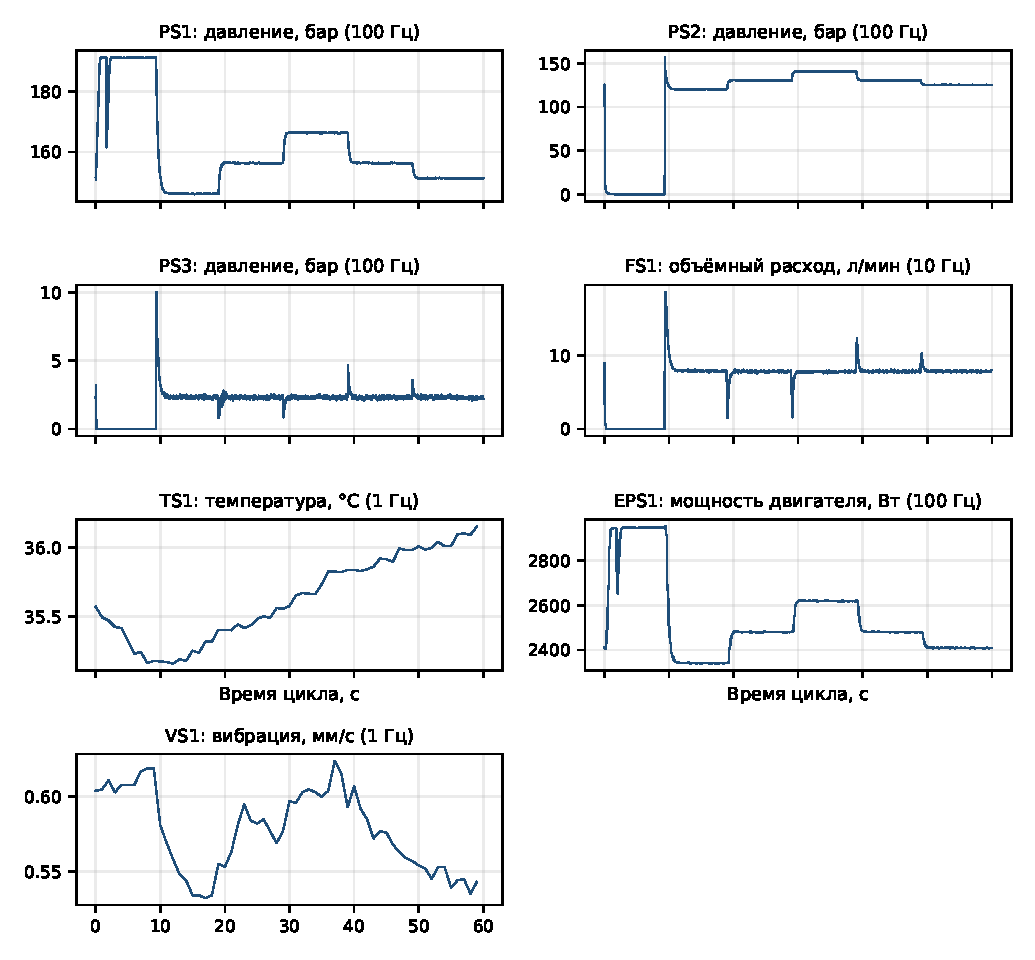
\includegraphics[width=0.92\textwidth]{figures/fig1_signals.pdf}
\caption{Один цикл стенда по семи каналам (начало кампании): ступенчатые
давления и мощность, медленная температура, высокочастотная вибрация}
\label{fig:signals}
\end{figure}

\subsection{Аудит: пропуски, константы, дубликаты, выбросы}

Результаты аудита собраны в таблицах~\ref{tab:data} и~\ref{tab:features}.
Пропусков нет, полных дубликатов строк нет, все \DataCycles{} строк
различимы. Два признака, \texttt{PS2\_min} и \texttt{PS3\_min}, постоянны на
всей кампании: минимальное давление в этих контурах упирается в одно и то же
значение. Ещё один признак, \texttt{FS1\_min}, почти постоянен (доля моды
превышает 0,999). Такие признаки после стандартизации дают либо деление на
ноль, либо огромные $z$-оценки и делают ковариационную матрицу в факторном
анализе вырожденной, поэтому из анализа исключены \DataNearConstant{} признака:
\texttt{\DataNearConstantList}. В работе остаётся \DataFeaturesUsed{} признак;
все \DataFeaturesAll{} описаны в таблице~\ref{tab:features}, исключённые
помечены звёздочкой.

\begin{table}[H]
\centering
\small
\caption{Характеристика набора данных и результаты аудита}
\label{tab:data}
\begin{tabular}{lr}
\toprule
Показатель & Значение \\
\midrule
Циклов (объектов) & \DataCycles \\
Каналов & \DataChannels \\
Циклопризнаков ($7 \times 4$) & \DataFeaturesAll \\
Признаков в анализе & \DataFeaturesUsed \\
Пропусков & \DataMissing \\
Полных дубликатов строк & \DataDuplicates \\
Постоянных признаков & \DataConstant \\
Малоинформативных, включая постоянные & \DataNearConstant \\
\midrule
Выбросов по правилу 1,5 IQR & \DataOutliers{} (\DataOutlierShare~\%) \\
Обучение: циклы & \DataTrainFirst--\DataTrainLast{} (\DataTrain) \\
Тест: циклы & \DataTestFirst--\DataTestLast{} (\DataTest) \\
Блочное разбиение: обучение / тест & \BlockTrain{} / \BlockTest \\
Длина блока & \BlockSize \\
\bottomrule
\end{tabular}
\end{table}

\begin{table}[!t]
\centering
\scriptsize
\renewcommand{\arraystretch}{0.93}
\caption{Циклопризнаки: единицы, диапазон, медиана, СКО, число выбросов и участие в анализе}\label{tab:features}
\resizebox{\textwidth}{!}{%
\begin{tabular}{llrrrrrr}
\toprule
Канал & Характеристика & Ед. & Мин. & Медиана & Макс. & СКО & Выбросы \\
\midrule
PS1 & среднее & бар & 155,39 & 158,96 & 180,92 & 4,6984 & 240 \\
PS1 & СКО & бар & 13,93 & 14,73 & 22,14 & 2,0675 & 240 \\
PS1 & минимум & бар & 133,13 & 143,31 & 146,69 & 2,1960 & 2 \\
PS1 & максимум & бар & 189,63 & 190,96 & 191,92 & 0,6028 & 0 \\
\midrule
PS2 & среднее & бар & 104,41 & 107,73 & 131,59 & 4,9854 & 240 \\
PS2 & СКО & бар & 45,20 & 46,80 & 59,55 & 3,2709 & 240 \\
PS2$^{\ast}$ & минимум & бар & 0,000 & 0,000 & 0,000 & 0,0000 & 0 \\
PS2 & максимум & бар & 155,04 & 166,65 & 167,77 & 0,9778 & 46 \\
\midrule
PS3 & среднее & бар & 0,840 & 1,780 & 2,023 & 0,2518 & 240 \\
PS3 & СКО & бар & 0,728 & 0,887 & 1,049 & 0,0398 & 8 \\
PS3$^{\ast}$ & минимум & бар & 0,000 & 0,000 & 0,000 & 0,0000 & 0 \\
PS3 & максимум & бар & 9,109 & 10,56 & 18,83 & 0,6397 & 3 \\
\midrule
FS1 & среднее & л/мин & 2,019 & 6,577 & 6,723 & 1,0326 & 240 \\
FS1 & СКО & л/мин & 2,664 & 2,982 & 3,739 & 0,1888 & 250 \\
FS1$^{\ast}$ & минимум & л/мин & 0,000 & 0,000 & 0,001 & 0,0000 & 1 \\
FS1 & максимум & л/мин & 18,70 & 20,36 & 20,48 & 0,4518 & 42 \\
\midrule
TS1 & среднее & °C & 35,31 & 44,84 & 57,90 & 7,9901 & 0 \\
TS1 & СКО & °C & 0,060 & 0,193 & 0,581 & 0,0443 & 33 \\
TS1 & минимум & °C & 34,98 & 44,45 & 57,38 & 7,9095 & 0 \\
TS1 & максимум & °C & 35,50 & 45,09 & 58,21 & 8,0198 & 0 \\
\midrule
EPS1 & среднее & Вт & 2361,75 & 2480,93 & 2740,64 & 73,82 & 10 \\
EPS1 & СКО & Вт & 185,09 & 196,14 & 294,02 & 27,76 & 241 \\
EPS1 & минимум & Вт & 2097,80 & 2260,00 & 2384,00 & 65,41 & 0 \\
EPS1 & максимум & Вт & 2813,40 & 2897,40 & 2995,20 & 49,64 & 0 \\
\midrule
VS1 & среднее & мм/с & 0,524 & 0,610 & 0,839 & 0,0602 & 5 \\
VS1 & СКО & мм/с & 0,013 & 0,032 & 0,461 & 0,0320 & 195 \\
VS1 & минимум & мм/с & 0,483 & 0,561 & 0,696 & 0,0408 & 3 \\
VS1 & максимум & мм/с & 0,562 & 0,689 & 2,546 & 0,1540 & 93 \\
\bottomrule
\end{tabular}}
\par\smallskip{\scriptsize $^{\ast}$Признак исключён из анализа: постоянный или почти постоянный.}
\end{table}


По правилу 1,5 интерквартильного размаха (IQR) помечено \DataOutliers{}
ячеек, то есть \DataOutlierShare~\% всех значений. Важно, что это не
равномерный шум: у средних давлений PS1--PS3 и расхода FS1 помечено ровно по
\DataHighPressN{} циклов (по \DataHighPressShare~\% кампании), и все они лежат
внутри отрезка \DataHighPressRange. Сравнение уровней показывает, что это
единый рабочий режим, а не случайные выбросы: на этих циклах давление PS1 в
среднем \HighFlagPsOne{} бар против \HighRestPsOne, расход \HighFlagFsOne~л/мин
против \HighRestFsOne, температура \HighFlagTsOne~°C против \HighRestTsOne,
мощность \HighFlagEpsOne~Вт против \HighRestEpsOne, а давление PS3, наоборот,
ниже (\HighFlagPsThree{} против \HighRestPsThree). Все \DataHighPressN{} циклов
относятся к состоянию охладителя «близко к отказу». Удалять их нельзя: это
содержательный режим, и ниже видно, что кластеризация находит его
самостоятельно (в подвыборке ему соответствуют ровно \DataHighPressSub{}
циклов~--- столько же, сколько объектов в первой группе KMeans).

На рисунке~\ref{fig:correlation} приведена матрица корреляций признаков.
Внутри одного канала среднее, минимум и максимум сильно коррелируют, а
стандартное отклонение часто ведёт себя иначе; между каналами выделяются
блоки «давления», «расход», «температура», «мощность» и «вибрация». Из-за
этих корреляций исходные \DataFeaturesUsed{} признаков содержат заметно
меньше независимых направлений, что и мотивирует снижение размерности.

\begin{figure}[!t]
\centering
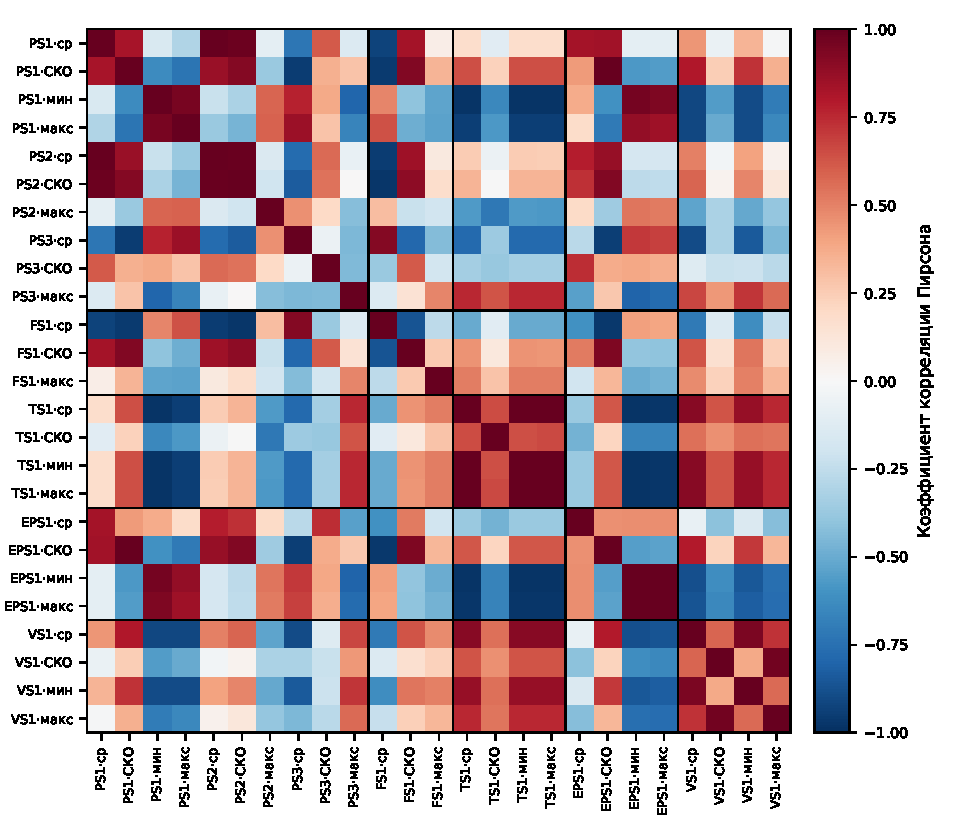
\includegraphics[width=0.78\textwidth]{figures/fig2_correlation.pdf}
\caption{Корреляции циклопризнаков; линии разделяют физические группы
каналов}
\label{fig:correlation}
\end{figure}

\subsection{Метки состояний}

Метки пяти показателей приведены в таблице~\ref{tab:labels}. Обращают на
себя внимание две особенности. Во-первых, состояния охладителя образуют три
почти равных блока по \CoolerPerLevel{}--\CoolerLast{} циклов: \texttt{3}
(близко к отказу), \texttt{20} (пониженная эффективность) и \texttt{100}
(полная эффективность). Во-вторых, уровень клапана \texttt{100} встречается
\ValveOptimal{} раз, а остальные три уровня~--- по \ValvePerLevel{} раз,
причём, как показано ниже, их доли одинаковы в начале, середине и конце
кампании. Это значит, что состояние клапана менялось независимо от времени, а
состояние охладителя~--- блоками. Такое различие принципиально для
интерпретации согласия кластеров с метками.

\begin{table}[!t]
\centering
\small
\caption{Уровни состояния узлов из \texttt{profile.txt} (в признаки не входят)}\label{tab:labels}
\begin{tabular}{llrr}
\toprule
Показатель & Уровень & $n$ & \% \\
\midrule
\multicolumn{4}{l}{\textit{Состояние охладителя, \%}} \\
 & 3: близко к отказу & 732 & 33,20 \\
 & 20: пониженная эффективность & 732 & 33,20 \\
 & 100: полная эффективность & 741 & 33,61 \\
\addlinespace
\multicolumn{4}{l}{\textit{Состояние клапана, \%}} \\
 & 73: близко к отказу & 360 & 16,33 \\
 & 80: сильное запаздывание & 360 & 16,33 \\
 & 90: слабое запаздывание & 360 & 16,33 \\
 & 100: оптимальное переключение & 1125 & 51,02 \\
\addlinespace
\multicolumn{4}{l}{\textit{Внутренняя утечка насоса}} \\
 & 0: нет утечки & 1221 & 55,37 \\
 & 1: слабая утечка & 492 & 22,31 \\
 & 2: сильная утечка & 492 & 22,31 \\
\addlinespace
\multicolumn{4}{l}{\textit{Давление гидроаккумулятора, бар}} \\
 & 90: близко к отказу & 808 & 36,64 \\
 & 100: сильно понижено & 399 & 18,10 \\
 & 115: слегка понижено & 399 & 18,10 \\
 & 130: оптимальное давление & 599 & 27,17 \\
\addlinespace
\multicolumn{4}{l}{\textit{Флаг установившегося режима}} \\
 & 0: режим установился & 1449 & 65,71 \\
 & 1: режим не установился & 756 & 34,29 \\
\bottomrule
\end{tabular}
\end{table}


\subsection{Два проверяемых вопроса}

Чтобы результат не сводился к перечислению графиков, заранее
сформулированы два вопроса, на которые в работе даётся ответ.

\textbf{Вопрос В1.} Является ли главная ось вариации физически однородной~---
например, чисто тепловой осью, связанной с эффективностью охладителя,~--- или
она смешивает тепловое состояние с медленным дрейфом кампании и потому не
может трактоваться как один физический фактор?

\textbf{Вопрос В2.} Образуют ли состояния клапана, гидроаккумулятора и насоса
отдельные группы в пространстве главных координат, или единственная
устойчивая структура~--- это деление кампании на временные блоки, совпадающие
с заменой охладителя?

Критерии ответа заданы до обращения к меткам. Для В1 смотрим на нагрузки
первой компоненты и на связь её счётов с номером цикла; для В2~--- на ARI
между найденными группами и уровнями узлов, на устойчивость разбиения и на
то, сохраняется ли согласие при смене масштаба.

% ============================================================================
\section{МЕТОДИКА}
% ============================================================================

\subsection{Разбиение и масштабирование}

Кампания упорядочена во времени, поэтому случайное разбиение строк дало бы
утечку: соседние циклы почти одинаковы, и ошибка на «отложенных» объектах
была бы занижена. Основное разбиение~--- хронологическое: обучение
\DataTrainFirst--\DataTrainLast{} (\DataTrain{} циклов), тест
\DataTestFirst--\DataTestLast{} (\DataTest). Все параметры преобразований
(средние, СКО, матрицы нагрузок, центроиды) оцениваются только на обучающей
части и применяются к тесту.

Дополнительно используется блочное разбиение: кампания режется на блоки по
\BlockSize{} последовательных циклов, блоки случайно делятся в пропорции
70/30, но целиком. Внутри блока соседние циклы остаются вместе, а состав
режимов сохраняется. Это более мягкая проверка: она отвечает на вопрос,
переносится ли модель на другие участки той же кампании, тогда как
хронологическое разбиение проверяет перенос в будущее.

Ограничения вычислительной нагрузки из условий задачи не являются
связывающими, но соблюдены: PCA выполнена на \DataCycles{} строках
(лимит 10\,000), факторный анализ~--- на \DataTrain{} (лимит 2\,000) и
\DataFeaturesUsed{} признаках (лимит 60), кластеризация~--- на \ClustN{}
(лимит 1\,200). t-SNE и Isomap не применялись: они не дают отображения новых
объектов и не нужны для ответа на поставленные вопросы.

\subsection{Метод главных компонент}

PCA~\cite{jolliffe} ищет ортогональные линейные комбинации признаков с
максимальной дисперсией. Рассмотрены два варианта предобработки:
\begin{itemize}
\item \emph{стандартизация}: каждый признак делится на своё СКО, все признаки
  становятся равноправными;
\item \emph{только центрирование}: признаки сохраняют единицы, и компоненты
  определяются абсолютными разбросами. Признак с большим разбросом (например,
  мощность в ваттах) доминирует.
\end{itemize}

Для $k = 1,\dots,10$ на тесте считается ошибка восстановления:
\[
\mathrm{RMSE}(k) = \sqrt{\frac{1}{n p}\sum_{i=1}^{n}\sum_{j=1}^{p}
\bigl(x_{ij} - \hat x_{ij}(k)\bigr)^2},
\]
где $\hat x = $ \texttt{inverse\_transform(transform(x))}. Абсолютная RMSE
смешивает единицы (ватты, бар, °C), поэтому дополнительно считается
относительная ошибка: RMSE по каждому признаку делится на его СКО на
обучающей части, затем значения усредняются. Знак каждой компоненты выбран
так, чтобы сумма нагрузок была положительной; это не меняет разбиения, но
делает таблицы и рисунки однозначными.

\subsection{Факторный анализ}

Факторный анализ~\cite{harman} описывает ковариационную матрицу как
$\Sigma = LL^{\top} + \Psi$, где $L$~--- нагрузки, а $\Psi$~--- диагональная
матрица шумовых дисперсий. В отличие от PCA, модель допускает
признак-специфический шум, а нагрузки на стандартизованных признаках равны
корреляциям с латентным фактором. Оценка~--- метод максимального
правдоподобия, до 2\,000 итераций, без вращения. Рассмотрены 2, 3 и 5
факторов; для каждого сохранены нагрузки, шумовые дисперсии
(\texttt{noise\_variance\_}), общности $1-\psi_j$ и среднее
лог-правдоподобие \texttt{score} на обучении, хронологическом тесте и
блочном тесте. Число факторов выбирается по правдоподобию на отложенных
циклах, а не по обучению.

\subsection{Кластеризация: одна подвыборка, одни координаты}

Сравнивать алгоритмы на разных пространствах бессмысленно, поэтому все три
метода работают на одной фиксированной подвыборке из \ClustN{} циклов
(\ClustShareOfAll~\% кампании, генератор с зерном 42) и на одних и тех же
координатах: первых \ClustPcs{} главных компонентах стандартизованного PCA,
которые объясняют \ClustSharePct~\% дисперсии. Сами координаты дополнительно
делятся на СКО по обучающей части, чтобы расстояние было евклидовым и
сопоставимым между компонентами.

Алгоритмы:
\begin{itemize}
\item KMeans~\cite{macqueen} с 20 запусками и выбором лучшего по инерции;
\item агломеративная кластеризация Уорда~\cite{ward} (минимизация прироста
  внутригрупповой суммы квадратов);
\item DBSCAN~\cite{ester} с фиксированным \texttt{min\_samples} и радиусом,
  выбранным по кривой расстояний до $k$-го соседа.
\end{itemize}

Для KMeans и Уорда перебраны $k = 2,\dots,6$. Качество измерялось силуэтом
\cite{rousseeuw} и индексом Дэвиса---Болдина \cite{davies}. Устойчивость
оценивалась по 20 бутстрэп-подвыборкам объёма 80~\%: алгоритм обучался
заново, а согласие с полным разбиением измерялось ARI~\cite{hubert} на общих
объектах. Среднее и стандартное отклонение ARI приведены в
таблице~\ref{tab:ksweep}.

\subsection{Правило выбора числа групп}

Правило выбора $k$ объявлено до обращения к меткам:
\begin{enumerate}
\item устойчивость не ниже \RuleStab;
\item каждая группа содержит не менее \RuleShare~\% объектов;
\item из оставшихся выбирается наименьшее $k$, силуэт которого не ниже
  \RuleSil~\% от максимального силуэта среди допустимых.
\end{enumerate}
Ограничение на размер группы отсекает вырожденные группы из нескольких
циклов, которые искусственно повышают силуэт. Порог \RuleSil~\% не позволяет
выбирать $k$ только из-за монотонного роста силуэта с числом групп. Метки
состояний в этом правиле не участвуют.

\subsection{DBSCAN}

Параметр \texttt{min\_samples} взят равным \DbMinSamples~(примерно удвоенная
размерность пространства). Радиус выбирался по $k$-distance: для каждой точки
считается расстояние до \DbMinSamples-го соседа, строится кривая этих
расстояний, и в качестве ориентира берётся 90-й процентиль
(\DbEpsRule). Из сетки $0{,}2$--$1{,}6$ с шагом $0{,}1$ выбирается
наименьший радиус не меньше ориентира, то есть $\varepsilon = \DbEps$.
Дополнительно проверена чувствительность к \texttt{min\_samples} = 5 и 20.

Силуэт и индекс Дэвиса---Болдина для DBSCAN считаются без точек шума, а доля
шума приводится отдельно: иначе метрика смешивала бы качество кластеров с
количеством отброшенных объектов. Для сравнения алгоритмов в
таблице~\ref{tab:clust} указаны и качество, и доля шума.

\subsection{Согласие с метками}

Метки используются только после того, как разбиения зафиксированы. Согласие
измеряется ARI (0~--- случайное разбиение, 1~--- совпадение) и NMI. Для
DBSCAN точки шума исключаются. ARI симметричен и не зависит от нумерации
групп, поэтому перенумерация групп по медианному номеру цикла (для
единообразия таблиц) на метрику не влияет.

Отдельно подчёркнуто: высокий ARI с меткой ещё не означает, что алгоритм
«нашёл неисправность». Если метка меняется блоками во времени, а кампания
дрейфует, то любая группировка по времени даст высокий ARI. Поэтому
согласие с охладителем сопоставляется с согласием с номером трети кампании и
с долями уровней по третям.

\subsection{Что не использовалось}

t-SNE и Isomap не применялись: они предназначены для визуализации и не
позволяют отобразить новый цикл без пересчёта, а вопрос о переносимости для
нас существен. NMF и FastICA не использовались: они добавляют предположения
(неотрицательность, независимость), которых в постановке нет, и не дают
сравнимой ошибки восстановления в исходных единицах. Обучение с учителем не
применялось, метки в признаки не попадали.

\subsection{Воспроизводимость}

Все случайные операции используют зерно 42. Одна команда
\texttt{python build.py} пересчитывает агрегаты (если распакованы исходные
каналы), строит все рисунки и таблицы, собирает PDF. Если исходных каналов
нет, используется проверенная таблица агрегатов, входящая в архив. Версии
библиотек зафиксированы в \texttt{requirements.txt}; текст отчёта не содержит
введённых вручную чисел~--- все они подставляются макросами из
\texttt{results.json}.

% ============================================================================
\section{СНИЖЕНИЕ РАЗМЕРНОСТИ: PCA И ФАКТОРНЫЙ АНАЛИЗ}
% ============================================================================

\subsection{Спектр и накопленная дисперсия}

На рисунке~\ref{fig:spectrum} и в таблице~\ref{tab:pca} приведены доли
объяснённой дисперсии. При стандартизации первая компонента объясняет
\PcaEvrOne, вторая~\PcaEvrTwo, третья~\PcaEvrThree, четвёртая~\PcaEvrFour;
две компоненты дают \PcaCumTwo, четыре~--- \PcaCumFour, шесть~---
\PcaCumSix, десять~--- \PcaCumTen. Резкого обрыва нет: после первых двух
компонент спектр спадает плавно, что типично для коррелированных, но не
низкоразмерных данных.

При только центрировании картина обманчиво проще: первая компонента
объясняет \PcaCentEvrOne, две~--- \PcaCentCumTwo, четыре~--- \PcaCentCumFour.
Выглядит так, будто данные почти двумерны. Это артефакт масштаба: нагрузка
первой компоненты почти целиком приходится на \texttt{EPS1\_mean}
(\PcaCentLoadEpsOne), потому что мощность в ваттах имеет на порядки больший
разброс, чем температура или давление. Компонента измеряет не «главную
физическую ось», а вариацию самого крупного по единицам признака. Поэтому
дальше как основное пространство используется стандартизованный вариант.

\begin{figure}[H]
\centering
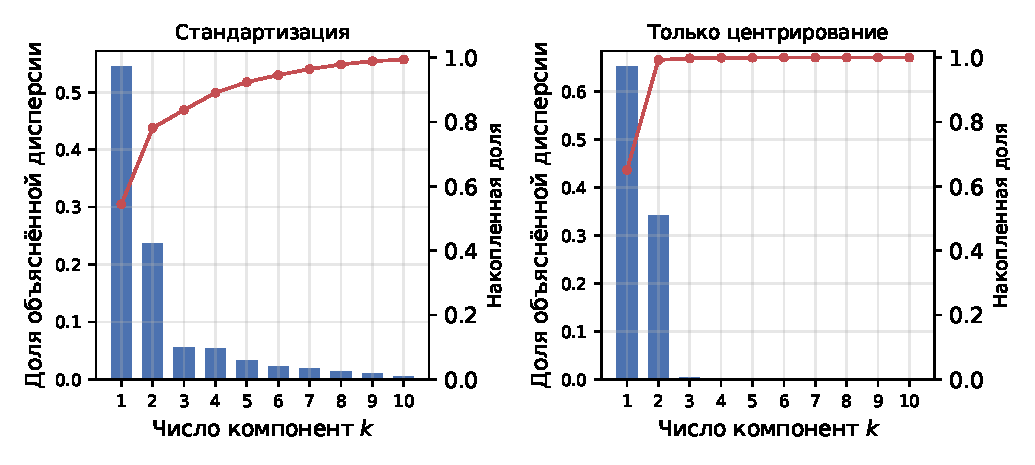
\includegraphics[width=\textwidth]{figures/fig4_spectrum.pdf}
\caption{Доли объяснённой дисперсии (столбцы) и накопленная доля (линия) при
стандартизации и только центрировании}
\label{fig:spectrum}
\end{figure}

\begin{table}[H]
\centering
\small
\caption{Доли объяснённой дисперсии PCA при стандартизации и только центрировании}\label{tab:pca}
\begin{tabular}{crrrr}
\toprule
$k$ & \multicolumn{2}{c}{Стандартизация} & \multicolumn{2}{c}{Центрирование} \\
\cmidrule(lr){2-3}\cmidrule(lr){4-5}
 & EVR & Накопл. & EVR & Накопл. \\
\midrule
1 & 0,5442 & 0,5442 & 0,6508 & 0,6508 \\
2 & 0,2373 & 0,7815 & 0,3419 & 0,9927 \\
3 & 0,0559 & 0,8374 & 0,0049 & 0,9976 \\
4 & 0,0532 & 0,8906 & 0,0018 & 0,9994 \\
5 & 0,0334 & 0,9240 & 0,0005 & 0,9999 \\
6 & 0,0218 & 0,9458 & 0,0001 & 0,9999 \\
7 & 0,0184 & 0,9643 & 0,0000 & 1,0000 \\
8 & 0,0144 & 0,9787 & 0,0000 & 1,0000 \\
9 & 0,0103 & 0,9889 & 0,0000 & 1,0000 \\
10 & 0,0049 & 0,9938 & 0,0000 & 1,0000 \\
\bottomrule
\end{tabular}
\end{table}


\subsection{Ошибка восстановления на отложенных циклах}

Ошибка восстановления (рисунок~\ref{fig:recon}, таблица~\ref{tab:recon})
показывает, сколько информации об исходных признаках теряется при сжатии.
При стандартизации относительная RMSE при $k=2$ равна \PcaRelStdTwo, при
$k=4$~--- \PcaRelStdFour, при $k=6$~--- \PcaRelStdSix, при $k=10$~---
\PcaRelStdTen. Абсолютная RMSE при $k=2$ составляет \PcaRmseStdTwo, но она
измерена в смеси единиц и приведена только для полноты. В таблице~5 она
немонотонна: абсолютная ошибка складывает потери разных признаков с разными
единицами, и при добавлении компоненты ошибка перераспределяется между ними.
Относительная ошибка в стандартизованном варианте убывает монотонно, поэтому
именно она используется для содержательных выводов.

Два вывода следуют из рисунка. Во-первых, ошибка падает медленно: чтобы
объяснить 90~\% дисперсии, нужно около четырёх компонент, но чтобы
восстановить признаки с относительной ошибкой ниже 20~\%, нужно около
десяти. Это согласуется с плавным спектром. Во-вторых, на блочном тесте
ошибка заметно выше, чем на хронологическом: при $k=2$ относительная RMSE
равна \PcaRelStdTwoBlocked{} против \PcaRelStdTwo. Причина~--- дрейф кампании:
блочное разбиение перемешивает ранние и поздние циклы, и подпространство,
построенное на одной смеси режимов, хуже описывает другую. Это первый
признак того, что структура данных нестационарна.

При центрировании абсолютная RMSE при $k=2$ равна \PcaRmseCentTwo, что
выглядит намного лучше, но относительная ошибка почти та же
(\PcaRelCentTwo), а на блочном тесте~--- \PcaRelCentTwoBlocked. Малое
абсолютное число объясняется тем, что центрированная PCA хорошо описывает
мощность (главный вклад в абсолютную ошибку) и плохо~--- остальные признаки.
Именно поэтому сравнивать варианты по абсолютной RMSE нельзя.

\begin{figure}[H]
\centering
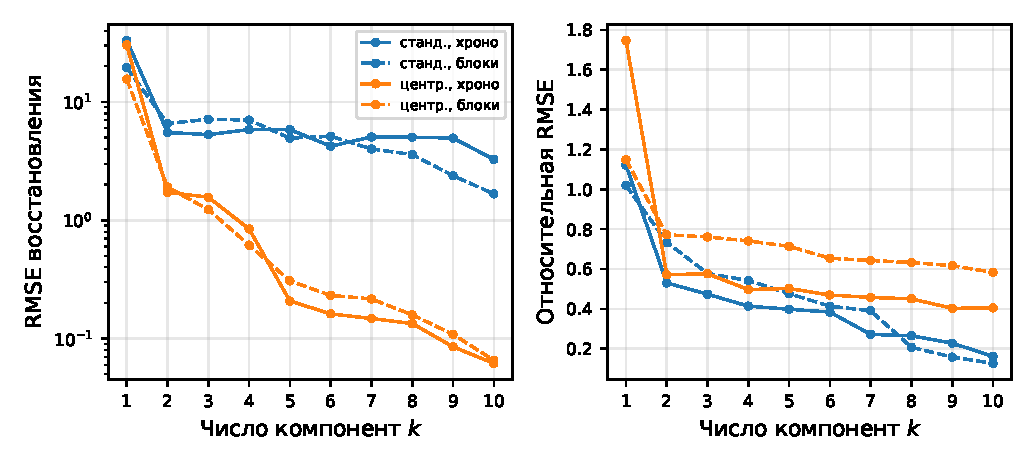
\includegraphics[width=\textwidth]{figures/fig5_reconstruction.pdf}
\caption{Ошибка восстановления на отложенных циклах: абсолютная (слева,
логарифмическая шкала) и относительная (справа) RMSE для хронологического и
блочного разбиений}
\label{fig:recon}
\end{figure}

\begin{table}[H]
\centering
\footnotesize
\caption{Ошибка восстановления PCA на отложенных циклах: RMSE в исходных единицах и относительная RMSE}\label{tab:recon}
\resizebox{\textwidth}{!}{%
\begin{tabular}{crrrrrr}
\toprule
$k$ & \multicolumn{3}{c}{Стандартизация} & \multicolumn{3}{c}{Центрирование} \\
\cmidrule(lr){2-4}\cmidrule(lr){5-7}
 & RMSE & Отн. (хроно) & Отн. (блоки) & RMSE & Отн. (хроно) & Отн. (блоки) \\
\midrule
1 & 33,08 & 1,121 & 1,020 & 30,33 & 1,747 & 1,148 \\
2 & 5,518 & 0,530 & 0,734 & 1,720 & 0,572 & 0,772 \\
3 & 5,296 & 0,474 & 0,578 & 1,564 & 0,576 & 0,761 \\
4 & 5,836 & 0,414 & 0,542 & 0,843 & 0,497 & 0,741 \\
5 & 5,831 & 0,398 & 0,476 & 0,207 & 0,502 & 0,714 \\
6 & 4,229 & 0,384 & 0,413 & 0,162 & 0,470 & 0,654 \\
7 & 5,053 & 0,272 & 0,390 & 0,147 & 0,457 & 0,643 \\
8 & 5,036 & 0,265 & 0,207 & 0,134 & 0,450 & 0,633 \\
9 & 4,949 & 0,228 & 0,158 & 0,085 & 0,403 & 0,617 \\
10 & 3,270 & 0,162 & 0,126 & 0,062 & 0,405 & 0,583 \\
\bottomrule
\end{tabular}}
\end{table}


\subsection{Нагрузки главных компонент}

Нагрузки первых четырёх компонент показаны на рисунке~\ref{fig:loadings}
слева. Первая компонента оказалась смешанной: в неё с сопоставимыми весами
входят вибрация \texttt{VS1\_mean} (\PcaLoadVsOne), давление \texttt{PS3\_mean}
(\PcaLoadPsThree), разброс давления \texttt{PS1\_std} (\PcaLoadPsOneStd), разброс
мощности \texttt{EPS1\_std} (\PcaLoadEpsOneStd), температура \texttt{TS1\_mean}
(\PcaLoadTsOne) и расход \texttt{FS1\_mean} (\PcaLoadFsOne). Это не одна
физическая величина, а комбинация «теплее, вибрация больше, давление в
третьем контуре ниже». Вторая компонента противопоставляет мощность и
давление температуре и вибрации: \texttt{EPS1\_mean} (\PcaLoadTwoEpsOne),
\texttt{PS1\_mean} (\PcaLoadTwoPsOne) и \texttt{PS2\_mean} (\PcaLoadTwoPsTwo) против
\texttt{TS1} (\PcaLoadTwoTsOne) и \texttt{VS1\_std} (\PcaLoadTwoVsOneStd). Третья и
четвёртая компоненты связаны в основном с экстремумами расхода и давления.

Таким образом, уже на уровне нагрузок видно, что главная ось не является
чисто тепловой. Ответ на вопрос В1 складывается из этого наблюдения и из
анализа дрейфа в разделе~5.

\begin{figure}[H]
\centering
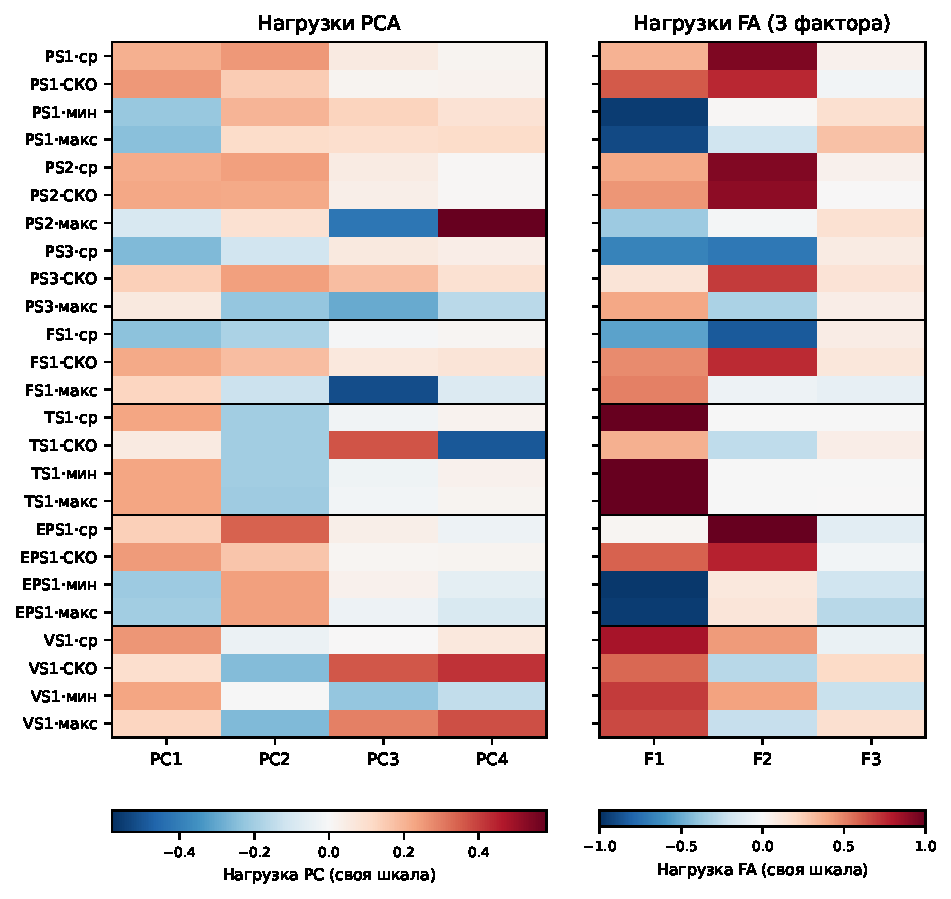
\includegraphics[width=0.95\textwidth]{figures/fig6_loadings.pdf}
\caption{Нагрузки PCA (слева, четыре компоненты) и факторного анализа
(справа, три фактора). Шкалы цветов у панелей свои; горизонтальные линии
разделяют физические группы каналов}
\label{fig:loadings}
\end{figure}

\subsection{Факторный анализ}

Результаты факторного анализа собраны в таблице~\ref{tab:fa} и на
рисунках~\ref{fig:loadings} (справа) и~\ref{fig:fa}. Среднее
лог-правдоподобие на обучении растёт с числом факторов
(\FaLlTrainTwo, \FaLlTrainThree, \FaLlTrainFive), что ожидаемо: больше
параметров~--- лучше подгонка. На хронологическом тесте лучшим оказывается
два фактора (\FaLlTestTwo{} против \FaLlTestThree{} и \FaLlTestFive), а на
блочном~--- пять (\FaLlBlockedFive{} против \FaLlBlockedTwo). Противоречие
между двумя тестами~--- ещё одно проявление нестационарности: разные части
кампании требуют разной сложности модели. По принципу бережливости выбран
вариант с двумя факторами; он же лучший на хронологическом тесте.

Средняя шумовая дисперсия при двух факторах \FaNoiseTwo, средняя общность
\FaCommTwo; при пяти факторах шум падает до \FaNoiseFive, а общность растёт
до \FaCommFive, но выигрыш на отложенных данных неоднозначен. Самые плохо
описываемые признаки~--- \texttt{TS1\_std} (\FaNoiseTsOneStd),
\texttt{PS3\_max} (\FaNoisePsThreeMax), \texttt{FS1\_max} (\FaNoiseFsOneMax) и
\texttt{VS1\_std} (\FaNoiseVsOneStd): их изменчивость почти не связана с общими
факторами.

Содержательно два фактора читаются отчётливо. Первый фактор~--- чистая
температурная ось: нагрузка \texttt{TS1\_mean} равна \FaLoadTsOne, а
\texttt{EPS1\_min} и \texttt{EPS1\_max}~--- \FaLoadEpsOneMin{} и
\FaLoadEpsOneMax. Второй фактор~--- мощность и давление: \texttt{EPS1\_mean}
\FaLoadTwoEpsOne, \texttt{PS1\_mean} \FaLoadTwoPsOne, \texttt{PS2\_mean}
\FaLoadTwoPsTwo, \texttt{FS1\_mean} \FaLoadTwoFsOne. Это физически осмысленная
картина: при нагреве меняются свойства жидкости и сопротивление контура,
поэтому температура и мощность/давление образуют две разные оси.

\begin{figure}[H]
\centering
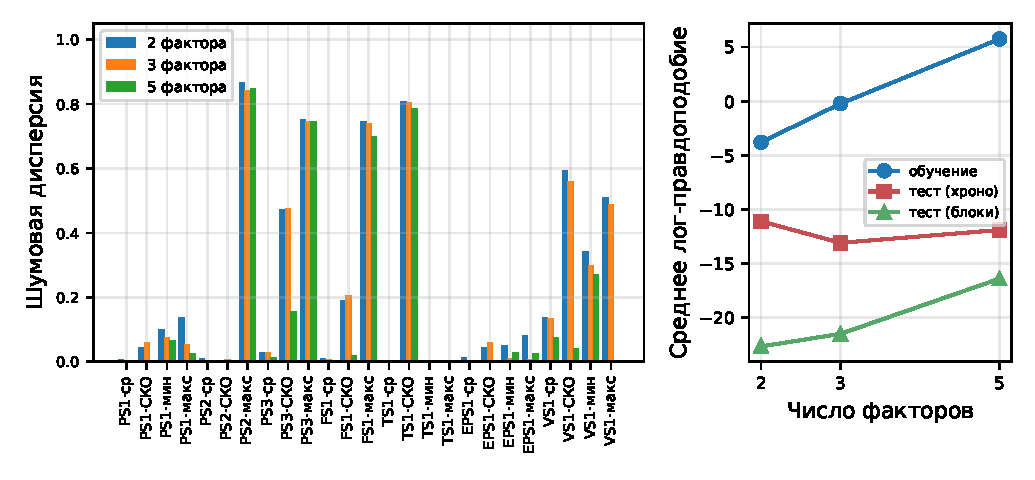
\includegraphics[width=\textwidth]{figures/fig7_fa.pdf}
\caption{Шумовая дисперсия признаков при 2, 3 и 5 факторах (слева) и среднее
лог-правдоподобие на обучении и двух отложенных разбиениях (справа)}
\label{fig:fa}
\end{figure}

\begin{table}[H]
\centering
\small
\caption{Факторный анализ: правдоподобие и остаточная структура}\label{tab:fa}
\resizebox{\textwidth}{!}{%
\begin{tabular}{crrrrrr}
\toprule
Факторов & LL (обучение) & LL (хроно-тест) & LL (блочный тест) & Средняя шум. дисп. & Средняя общность & Итераций \\
\midrule
2 & \textminus{}3,79 & \textminus{}11,09 & \textminus{}22,65 & 0,238 & 0,762 & 286 \\
3 & \textminus{}0,22 & \textminus{}13,08 & \textminus{}21,48 & 0,224 & 0,776 & 443 \\
5 & 5,75 & \textminus{}11,89 & \textminus{}16,39 & 0,153 & 0,847 & 482 \\
\bottomrule
\end{tabular}}
\end{table}


\subsection{Чем PCA отличается от факторного анализа в этом наборе}

Различие не только формальное. PCA максимизирует дисперсию и не содержит
модели шума: любая изменчивость, включая шум датчика, увеличивает
объяснённую дисперсию. Поэтому первая компонента собирает вклады многих
признаков и не обязана быть физически однородной. Факторный анализ, наоборот,
объясняет только коррелированную часть, а индивидуальный разброс относит в
$\Psi$. В результате его факторы получаются «чище»: F1 почти совпадает с
температурой, F2~--- с мощностью и давлением. Плата за это~--- предположение
о нормальности и диагональности шума, а также неоднозначность вращения:
нагрузки определены с точностью до ортогонального преобразования, поэтому
сравнивать их с PCA можно только качественно.

Практический вывод: для сжатия и восстановления признаков удобнее PCA (есть
явная ошибка в исходных единицах), для интерпретации осей~--- факторный
анализ.

% ============================================================================
\section{КЛАСТЕРИЗАЦИЯ}
% ============================================================================

\subsection{Перебор числа групп и устойчивость}

На рисунке~\ref{fig:kselect} и в таблице~\ref{tab:ksweep} показаны силуэт и
устойчивость для KMeans и Уорда. Силуэт у KMeans немонотонен: \KmSilTwo{} при
$k=2$, \KmSil{} при $k=3$, \KFourSil{} при $k=4$, \KFiveSil{} при $k=5$ и
\KSixSil{} при $k=6$. Рост после $k=4$ обманчив: при $k=5$ появляется группа
из \KFiveSizeMin{} объектов, при $k=6$~--- из \KSixSizeMin. Такие группы
отделены от остальных почти тривиально и повышают средний силуэт, не описывая
никакого нового режима.

По объявленному правилу отбрасываются $k=5$ и $k=6$ (группы меньше
\RuleShare~\% объектов). Среди $k=2,3,4$ максимальный силуэт у $k=3$
(\KmSil), поэтому порог составляет 95~\% от максимального силуэта, то есть
$0{,}95 \cdot \KmSil$; $k=2$ с силуэтом \KmSilTwo{}
не проходит, $k=4$ с \KFourSil{} проходит, и выбирается наименьшее
подходящее~--- $k=\KmK$. Устойчивость выбранного разбиения \KmStab, то есть
при бутстрэпе группы воспроизводятся практически без изменений.

\begin{figure}[H]
\centering
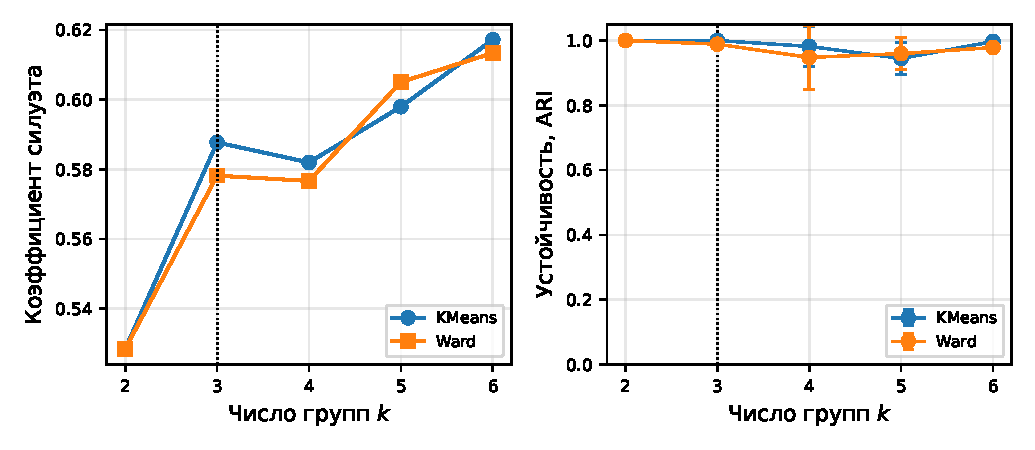
\includegraphics[width=\textwidth]{figures/fig8_k_selection.pdf}
\caption{Силуэт (слева) и устойчивость по бутстрэпу (справа) для KMeans и
Уорда; пунктир~--- выбранное $k$}
\label{fig:kselect}
\end{figure}

\begin{table}[H]
\centering
\scriptsize
\caption{Перебор числа групп: размеры (по убыванию), силуэт, Дэвис---Болдин, устойчивость и совпадение с состоянием охладителя}\label{tab:ksweep}
\resizebox{\textwidth}{!}{%
\begin{tabular}{crrrrrrrrrr}
\toprule
 & \multicolumn{5}{c}{KMeans} & \multicolumn{5}{c}{Ward} \\
\cmidrule(lr){2-6}\cmidrule(lr){7-11}
$k$ & Размеры & Силуэт & Д.--Б. & Устойч. & ARI охл. & Размеры & Силуэт & Д.--Б. & Устойч. & ARI охл. \\
\midrule
2 & 802/398 & 0,528 & 0,674 & 1,000 & 0,565 & 802/398 & 0,528 & 0,674 & 1,000 & 0,565 \\
3 & 675/398/127 & 0,588 & 0,634 & 1,000 & 0,582 & 684/398/118 & 0,578 & 0,604 & 0,989 & 0,577 \\
4 & 412/398/263/127 & 0,582 & 0,822 & 0,982 & 0,879 & 409/398/275/118 & 0,577 & 0,851 & 0,948 & 0,890 \\
5 & 417/398/247/127/11 & 0,598 & 0,692 & 0,945 & 0,855 & 409/398/189/118/86 & 0,605 & 0,791 & 0,960 & 0,834 \\
6 & 408/398/188/125/69/12 & 0,617 & 0,619 & 0,997 & 0,829 & 409/398/179/118/86/10 & 0,613 & 0,665 & 0,978 & 0,828 \\
\bottomrule
\end{tabular}}
\end{table}


\subsection{Иерархическая кластеризация и дендрограмма}

Уорд даёт почти то же разбиение, что и KMeans: при $k=3$ группы
\WardSizeOne, \WardSizeTwo{} и \WardSizeThree{} против \KmSizeOne, \KmSizeTwo{}
и \KmSizeThree, ARI между разбиениями \KmAriAg, силуэт \WardSil, индекс
Дэвиса---Болдина \WardDb, устойчивость \WardStab. Совпадение не случайно:
оба метода минимизируют внутригрупповой разброс, только один жадно, а другой
через последовательные слияния.

Дендрограмма на 80 случайных циклах и кривая расстояний последних слияний
приведены на рисунке~\ref{fig:dendro}. На дендрограмме видны три крупные
ветви; на кривой расстояний есть заметный перепад перед переходом от трёх
групп к двум, после которого расстояния растут плавно. Это независимое
подтверждение того, что $k=3$~--- разумный масштаб укрупнения, хотя сам
перепад не настолько резкий, чтобы говорить о «истинном» числе режимов.

\begin{figure}[H]
\centering
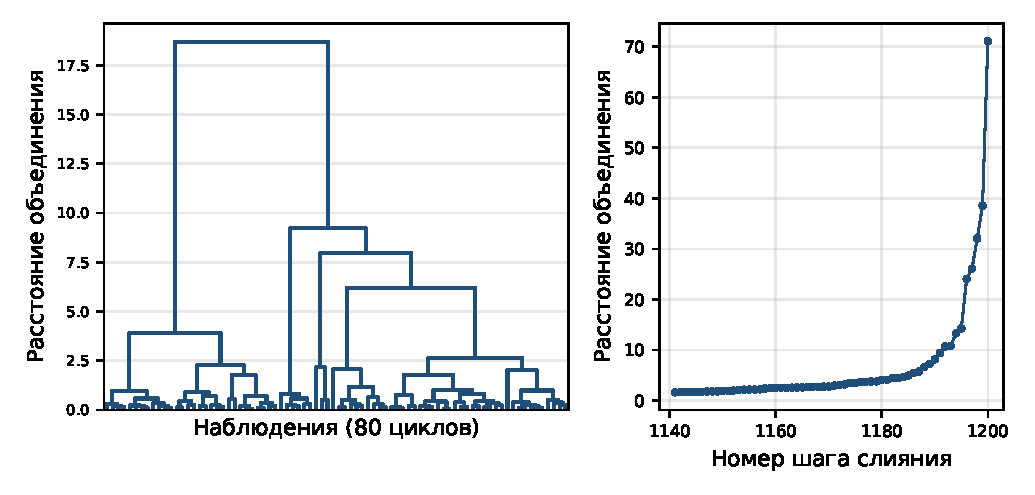
\includegraphics[width=\textwidth]{figures/fig10_dendrogram.pdf}
\caption{Дендрограмма Уорда на 80 циклах (слева) и расстояния последних
слияний для полной подвыборки (справа)}
\label{fig:dendro}
\end{figure}

\subsection{DBSCAN}

Кривая расстояний до $k$-го соседа приведена на рисунке~\ref{fig:kdist}.
Ориентир по 90-му процентилю равен \DbEpsRule, поэтому выбран
$\varepsilon = \DbEps$. При этом радиусе получается \DbNClusters{} группы
размеров \DbSizeOne/\DbSizeTwo/\DbSizeThree/\DbSizeFour, доля шума
\DbNoise~\%. Силуэт без шума \DbSil, индекс Дэвиса---Болдина \DbDb.

Чувствительность видна из таблицы~\ref{tab:dbscan}. При малых радиусах
($0{,}2$--$0{,}5$) группы те же, но доля шума растёт до \DbNoiseSmall~\%:
алгоритм отбрасывает разреженные переходные циклы. При
$\varepsilon \ge 0{,}7$ ранние две группы сливаются в одну, и остаётся три
кластера; при $\varepsilon = 1{,}6$ сливаются уже средняя и поздняя группы.
Выбранный $\varepsilon = \DbEps$~--- последнее значение, при котором ещё
различаются неустановившийся и стационарный участки раннего блока. При
\texttt{min\_samples} = 5 доля шума \DbMsFiveNoise~\%, при 20~---
\DbMsTwentyNoise~\%, а число групп меняется слабо, то есть результат умеренно
чувствителен к параметру.

\begin{figure}[H]
\centering
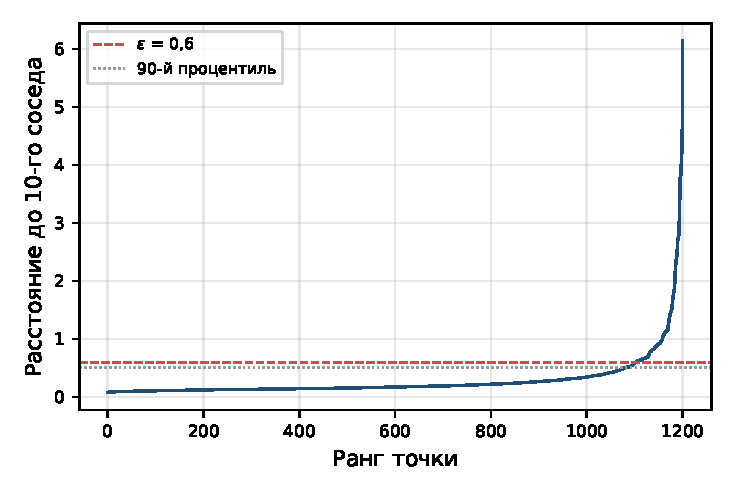
\includegraphics[width=0.72\textwidth]{figures/fig9_kdist.pdf}
\caption{Расстояния до 10-го соседа, отсортированные по возрастанию; линии
отмечают выбранный радиус и 90-й процентиль}
\label{fig:kdist}
\end{figure}

\begin{table}[H]
\centering
\small
\caption{Зависимость разбиения DBSCAN от радиуса $\varepsilon$ при \texttt{min\_samples}~=~10}\label{tab:dbscan}
\begin{tabular}{crrrr}
\toprule
$\varepsilon$ & Групп & Доля шума, \% & Силуэт & Д.--Б. \\
\midrule
0,2 & 4 & 27,1 & 0,710 & 0,363 \\
0,3 & 4 & 15,3 & 0,681 & 0,473 \\
0,4 & 4 & 9,1 & 0,656 & 0,561 \\
0,5 & 4 & 7,2 & 0,646 & 0,587 \\
\textbf{0,6} & 4 & 5,0 & 0,635 & 0,618 \\
0,7 & 3 & 3,8 & 0,632 & 0,519 \\
0,8 & 3 & 3,2 & 0,625 & 0,529 \\
0,9 & 3 & 2,5 & 0,619 & 0,539 \\
1,0 & 3 & 2,2 & 0,616 & 0,542 \\
1,1 & 3 & 2,0 & 0,613 & 0,547 \\
1,2 & 3 & 1,5 & 0,611 & 0,562 \\
1,3 & 3 & 1,3 & 0,608 & 0,566 \\
1,4 & 3 & 1,3 & 0,608 & 0,566 \\
1,5 & 3 & 1,1 & 0,606 & 0,580 \\
1,6 & 2 & 1,1 & 0,392 & 0,754 \\
\bottomrule
\end{tabular}
\end{table}


\subsection{Сравнение трёх разбиений}

Итоговое сравнение приведено в таблице~\ref{tab:clust}, а сами разбиения~---
на рисунке~\ref{fig:clusters}. Все три метода видят одну и ту же крупную
структуру: ранний блок с охладителем \texttt{3}, средний с \texttt{20} и
поздний с \texttt{100}. Различия касаются дробности.

KMeans и Уорд дают по три группы практически одинакового состава
(\KmSizeOne, \KmSizeTwo, \KmSizeThree{} у KMeans и \WardSizeOne, \WardSizeTwo,
\WardSizeThree{} у Уорда). DBSCAN выделяет четыре группы и дополнительно относит
\DbNoise~\% циклов к шуму. За счёт этого его силуэт (\DbSil) выше, чем у
KMeans (\KmSil), но сравнивать эти числа нужно осторожно: силуэт DBSCAN
посчитан без \DbNoise~\% наиболее разреженных точек. Индекс
Дэвиса---Болдина у DBSCAN \DbDb, у KMeans \KmDb, у Уорда \WardDb~---
величины одного порядка.

Согласие разбиений: ARI KMeans--Уорд \KmAriAg, ARI KMeans--DBSCAN \KmAriDb.
То есть DBSCAN не просто «дробит иначе», а действительно отделяет часть
раннего блока. По профилям (приложение~Б) видно, что это за часть: группа
DBSCAN~1 (\DbSizeOne{} циклов, \DbStableOne~\% неустановившихся)~--- это
переходный режим в начале кампании, а группа DBSCAN~2 (\DbSizeTwo,
\DbStableTwo~\% неустановившихся)~--- стационарная часть того же блока с
охладителем \texttt{3}.

\begin{figure}[H]
\centering
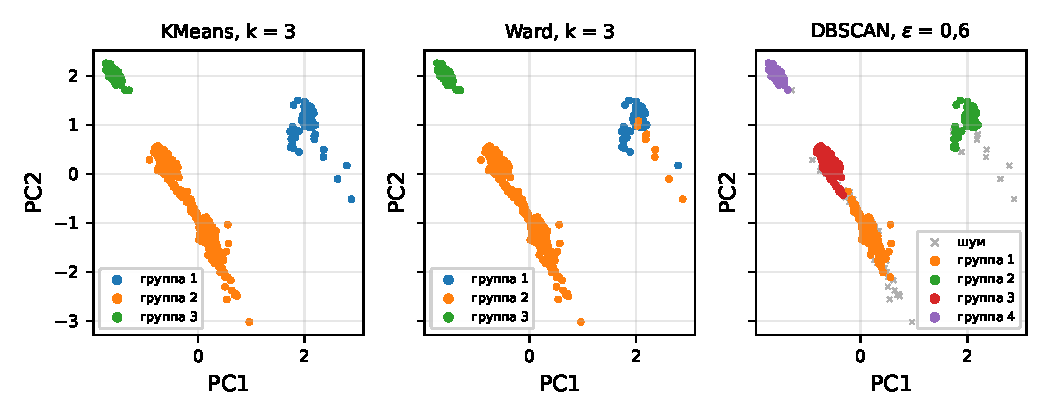
\includegraphics[width=\textwidth]{figures/fig11_clusters.pdf}
\caption{Разбиения KMeans, Уорда и DBSCAN в плоскости PC1--PC2; точки шума
DBSCAN показаны крестиками}
\label{fig:clusters}
\end{figure}

\begin{table}[H]
\centering
\footnotesize
\caption{Сравнение трёх алгоритмов на одной подвыборке 1~200 циклов и четырёх PCA-координатах}\label{tab:clust}
\resizebox{\textwidth}{!}{%
\begin{tabular}{lcrrrrrrr}
\toprule
Алгоритм & Групп & Размеры групп & Силуэт & Д.--Б. & Шум, \% & ARI охл. & ARI клап. & ARI акк. \\
\midrule
KMeans & 3 & 127/675/398 & 0,588 & 0,634 & 0,0 & 0,582 & 0,038 & 0,039 \\
Ward & 3 & 118/684/398 & 0,578 & 0,604 & 0,0 & 0,577 & 0,035 & 0,035 \\
DBSCAN & 4 & 224/114/405/397 & 0,635 & 0,618 & 5,0 & 0,906 & 0,013 & 0,096 \\
\bottomrule
\end{tabular}}
\end{table}


\subsection{Профили групп}

Профили всех групп собраны в приложении~Б (таблица~\ref{tab:profile}).
Группы перенумерованы по возрастанию медианного номера цикла, поэтому
«группа~1» везде ранняя, «группа~3» (или 4)~--- поздняя.

У KMeans группа~1 (\KmSizeOne{} циклов, \KmCycleOne) на 100~\% состоит из
циклов с охладителем \texttt{3} и почти не содержит неустановившихся режимов
(\KmStableOne~\%). Группа~2 (\KmSizeTwo, \KmCycleTwo) смешанная: в ней
\KmGTwoCoolerThree{} циклов с охладителем \texttt{3}, \KmGTwoCoolerTwenty~--- с
\texttt{20} и лишь \KmGTwoCoolerHundred{} с \texttt{100}; доля
неустановившихся \KmStableTwo~\%~--- самая высокая. Группа~3 (\KmSizeThree,
\KmCycleThree) целиком состоит из охлаждения \texttt{100}
(\KmGThreeCoolerHundred{} циклов) и на \KmStableThree~\% не установилась.

Иными словами, KMeans режет кампанию не на три равных блока, а иначе:
ранний блок делится на «нагруженный» участок (\KmSizeOne) и остальную часть,
которая объединяется со средним блоком. Именно поэтому ARI с охладителем
(\KmAriCooler) заметно ниже единицы, хотя состав групп по охладителю почти
чистый.

У Уорда профили те же с точностью до нескольких циклов. У DBSCAN четыре
группы: \DbSizeOne{} (\DbCycleOne, \DbStableOne~\% неустановившихся),
\DbSizeTwo{} (\DbCycleTwo, \DbStableTwo~\%), \DbSizeThree{} (\DbCycleThree)
и \DbSizeFour{} (\DbCycleFour). Третья группа почти целиком соответствует
охладителю \texttt{20}, четвёртая~--- \texttt{100}.

% ============================================================================
\section{СОПОСТАВЛЕНИЕ С МЕТКАМИ И ДРЕЙФ КАМПАНИИ}
% ============================================================================

\subsection{Согласие с состоянием охладителя}

Согласие с метками приведено в таблице~\ref{tab:match}, матрицы
сопряжённости~--- в приложении~А и на рисунке~\ref{fig:crosstab}, а
распределение меток в плоскости PC1--PC2~--- на рисунке~\ref{fig:labelplane}.

ARI с охладителем у KMeans \KmAriCooler, у Уорда \WardAriCooler, у DBSCAN
\DbAriCooler; NMI соответственно \KmNmiCooler, \WardNmiCooler{} и
\DbNmiCooler. Формально DBSCAN почти восстанавливает метку. Однако сравнение
с таблицей~\ref{tab:drift} показывает, что метка охладителя меняется блоками:
\CoolerPerLevel{} циклов \texttt{3}, затем 732 цикла \texttt{20}, затем
\CoolerLast{} цикла \texttt{100}. Эти блоки почти совпадают с третями
кампании. Значит, высокий ARI отражает прежде всего то, что и метка, и
кластеры упорядочены во времени; приписывать его «диагностике неисправности
охладителя» нельзя.

Тем не менее не всё сводится к времени. KMeans при $k=3$ даёт группу~1,
целиком состоящую из охлаждения \texttt{3}, но занимающую только часть
раннего блока; группа при $k=4$ (ARI \KFourAriCooler) ещё точнее совпадает
с меткой. То есть внутри блока \texttt{3} данные различают подобласти, и это
уже не временное деление. DBSCAN идёт дальше и выделяет переходный участок с
долей неустановившихся \DbStableOne~\%, именно за счёт этого его ARI выше.

\begin{figure}[H]
\centering
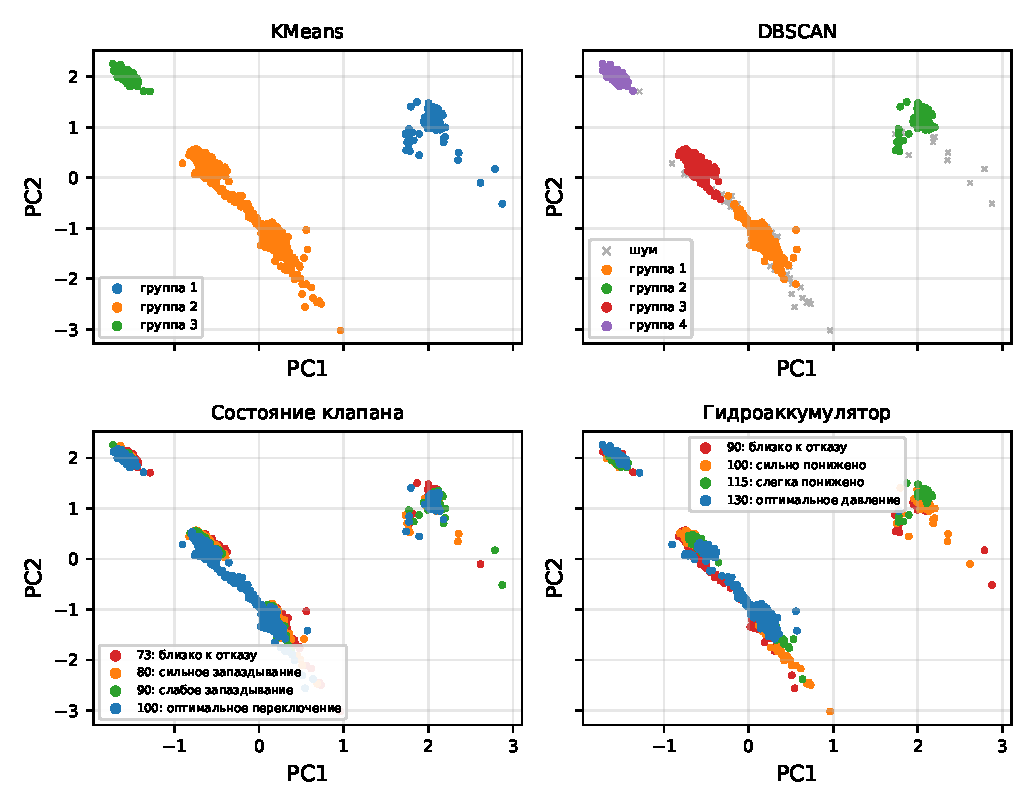
\includegraphics[width=0.95\textwidth]{figures/fig12_label_plane.pdf}
\caption{Разбиения KMeans и DBSCAN и метки клапана и гидроаккумулятора в
плоскости PC1--PC2}
\label{fig:labelplane}
\end{figure}

\begin{table}[H]
\centering
\small
\caption{Согласие найденных групп с состояниями узлов: ARI / NMI (для DBSCAN без точек шума)}\label{tab:match}
\begin{tabular}{lrrr}
\toprule
Состояние & KMeans & Ward & DBSCAN \\
\midrule
Охладитель & 0,582 / 0,702 & 0,577 / 0,699 & 0,906 / 0,915 \\
Клапан & 0,038 / 0,014 & 0,035 / 0,013 & 0,013 / 0,015 \\
Насос & 0,096 / 0,070 & 0,104 / 0,090 & 0,051 / 0,095 \\
Гидроаккумулятор & 0,039 / 0,053 & 0,035 / 0,049 & 0,096 / 0,113 \\
\bottomrule
\end{tabular}
\end{table}


\subsection{Клапан, насос и гидроаккумулятор}

С этими узлами картина другая. ARI с клапаном у KMeans \KmAriValve, у
Уорда \WardAriValve, у DBSCAN \DbAriValve; NMI не превышает \NmiValveMax.
Иными словами, найденные группы не несут информации об уровне клапана. Это
согласуется с тем, что доли уровней клапана одинаковы во всех третях
кампании: по \DriftValveEach~\% на уровни 73, 80 и 90 и
\DriftValveOptimal~\% на уровень 100 в каждой трети. Клапан менялся
независимо от времени, и в пространстве циклопризнаков его состояния не
образуют компактных областей.

С насосом ARI \KmAriPump, с гидроаккумулятором \KmAriAccum; у DBSCAN
соответственно \DbAriPump{} и \DbAriAccum. Это близко к случайному уровню.
Для гидроаккумулятора, правда, виден временной сдвиг: доля давления 90 бар
растёт с \DriftAccumNinetyEarly~\% в ранней трети до \DriftAccumNinetyMid~\%
и \DriftAccumNinetyLate~\% в средней и поздней. Но этот сдвиг не превращается
в отдельную группу, потому что он мал по сравнению с тепловым и нагрузочным
разбросом.

На рисунке~\ref{fig:labelplane} видно, что точки, окрашенные по уровню
клапана, перемешаны внутри каждой группы, а уровни гидроаккумулятора
образуют слабые полосы, не совпадающие с границами кластеров. Это
отрицательный, но важный результат: на уровне циклопризнаков состояния этих
узлов не разделяются.

\begin{figure}[H]
\centering
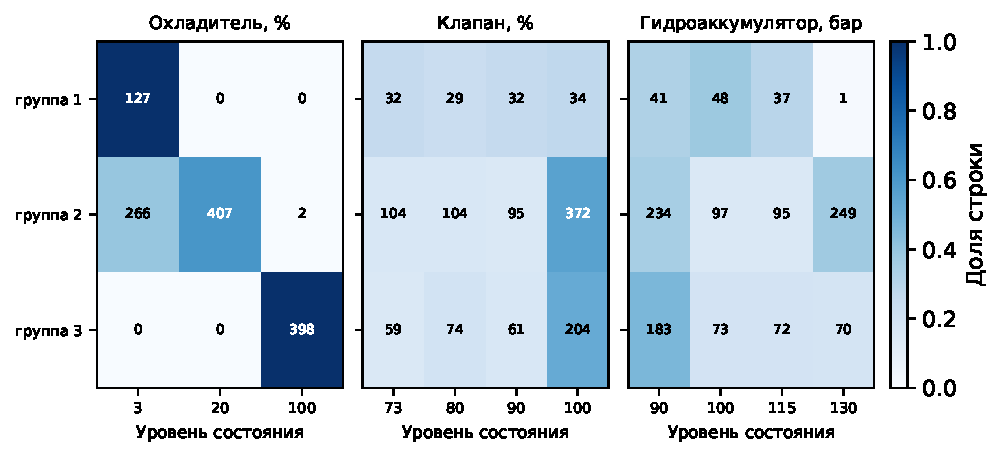
\includegraphics[width=\textwidth]{figures/fig13_crosstab.pdf}
\caption{Доли уровней состояний внутри групп KMeans; числа~--- количества
циклов подвыборки}
\label{fig:crosstab}
\end{figure}

\subsection{Дрейф кампании}

Таблица~\ref{tab:drift} и рисунок~\ref{fig:drift} показывают, что кампания
нестационарна. Средняя температура за цикл падает с \DriftTsOneEarly~°C в
ранней трети до \DriftTsOneMid~°C в средней и \DriftTsOneLate~°C в поздней;
вибрация~--- с \DriftVsOneEarly{} до \DriftVsOneMid{} и \DriftVsOneLate{} мм/с;
мощность, наоборот, к концу растёт (\DriftEpsOneEarly, \DriftEpsOneMid,
\DriftEpsOneLate~Вт). Средний счёт по первой компоненте меняется с
\DriftPcOneEarly{} до \DriftPcOneMid{} и \DriftPcOneLate.

Связь первой компоненты с номером цикла количественно велика: коэффициент
корреляции Пирсона \DriftPcOneCorr, Спирмена \DriftPcOneSpearman. Самые сильные
связи со временем у \texttt{\DriftTopFeature} (\DriftTopCorr) и
\texttt{\DriftSecondFeature} (\DriftSecondCorr). Это означает, что
«главная ось» в значительной мере является осью времени кампании, а не
только осью состояния охладителя. Ответ на вопрос В1, таким образом,
отрицательный: первая компонента смешивает тепловое состояние и дрейф.

Доли групп по третям (таблица~\ref{tab:drift}) подтверждают это: в ранней
трети \DriftGroupOneEarly~\% объектов попадает в группу~1 и
\DriftGroupTwoEarly~\%~--- в группу~2; в средней все объекты попадают в
группу~2 (\DriftGroupTwoMid~\%); в поздней \DriftGroupThreeLate~\% в группе~3.
Кластеры почти совпадают с третями, но не полностью: разделение ранней
трети на группы 1 и 2~--- единственное место, где структура не сводится к
календарю.

\begin{figure}[H]
\centering
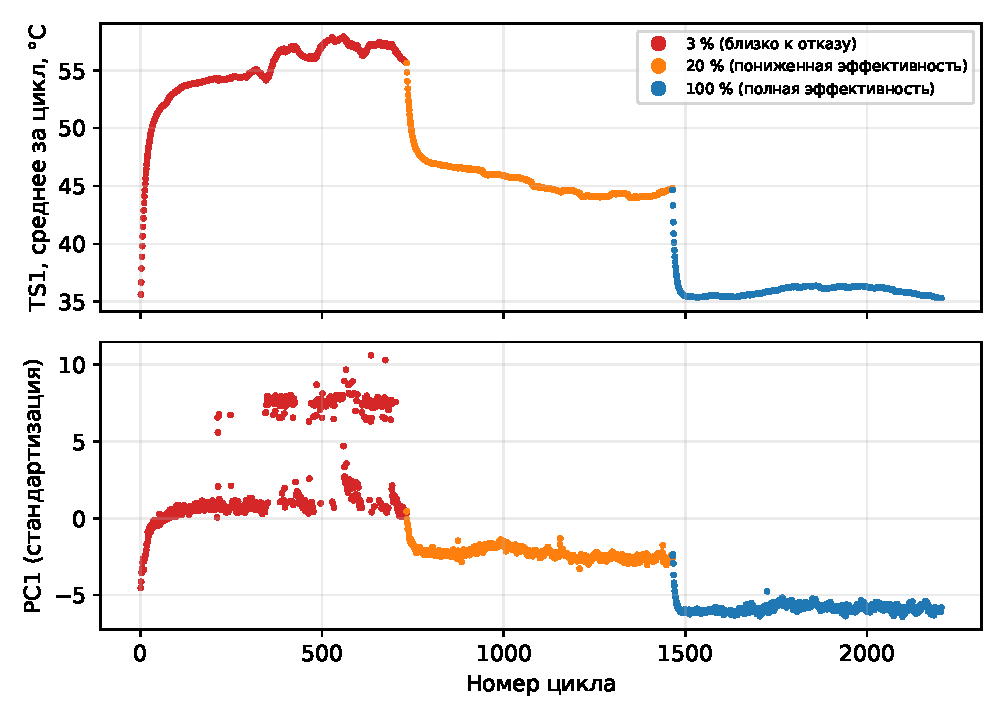
\includegraphics[width=0.95\textwidth]{figures/fig3_drift.pdf}
\caption{Температура TS1 (сверху) и счёт по первой компоненте (снизу) вдоль
кампании; цвет~--- состояние охладителя}
\label{fig:drift}
\end{figure}

\begin{table}[H]
\centering
\small
\caption{Ранняя, средняя и поздняя трети кампании (доли групп — по подвыборке 1~200 циклов)}\label{tab:drift}
\begin{tabular}{lrrr}
\toprule
Показатель & Ранняя & Средняя & Поздняя \\
\midrule
Циклы & 1--735 & 736--1470 & 1471--2205 \\
\midrule
TS1, среднее, $^\circ$C & 54,960 & 45,405 & 35,908 \\
VS1, среднее, мм/с & 0,680 & 0,611 & 0,549 \\
EPS1, среднее, Вт & 2473,759 & 2463,392 & 2549,377 \\
PS1, среднее, бар & 162,129 & 158,496 & 160,831 \\
PC1, среднее & 2,87 & \textminus{}2,27 & \textminus{}5,85 \\
\midrule
Доля группы 1 (KMeans), \% & 32,2 & 0,0 & 0,0 \\
Доля группы 2 (KMeans), \% & 67,8 & 100,0 & 0,0 \\
Доля группы 3 (KMeans), \% & 0,0 & 0,0 & 100,0 \\
\midrule
Доля охладителя 3, \% & 99,6 & 0,0 & 0,0 \\
Доля охладителя 20, \% & 0,4 & 99,2 & 0,0 \\
Доля охладителя 100, \% & 0,0 & 0,8 & 100,0 \\
\bottomrule
\end{tabular}
\end{table}


\subsection{Чувствительность к координатам и масштабу}

Наконец, проверено, насколько вывод зависит от выбранного пространства
(рисунок~\ref{fig:sens}, таблица~\ref{tab:sensitivity}). Силуэт KMeans при
$k=3$ равен \SensSilPcFourZ{} на четырёх стандартизованных компонентах,
\SensSilPcFourRaw{} без $z$-масштабирования, \SensSilPcTwoZ{} на двух
компонентах, \SensSilRawZ{} на \DataFeaturesUsed{} стандартизованных
признаках, \SensSilRawRaw{} на исходных признаках и \SensSilPcFourCentZ{} на
центрированных компонентах.

Разброс силуэта велик (от \SensSilPcFourCentZ{} до \SensSilPcTwoZ), но
состав групп почти не меняется: ARI с охладителем равен
\SensAriCoolerPcFourZ{} во всех вариантах, кроме варианта на исходных
признаках, где он \SensAriCoolerRawRaw. Это важный вывод: силуэт нельзя
сравнивать между разными масштабами, а устойчивость содержательного
результата~--- можно. Именно поэтому в работе фиксировано одно пространство
(четыре стандартизованные компоненты), а чувствительность приводится как
проверка, а не как способ выбрать «лучший» силуэт.

\begin{figure}[H]
\centering
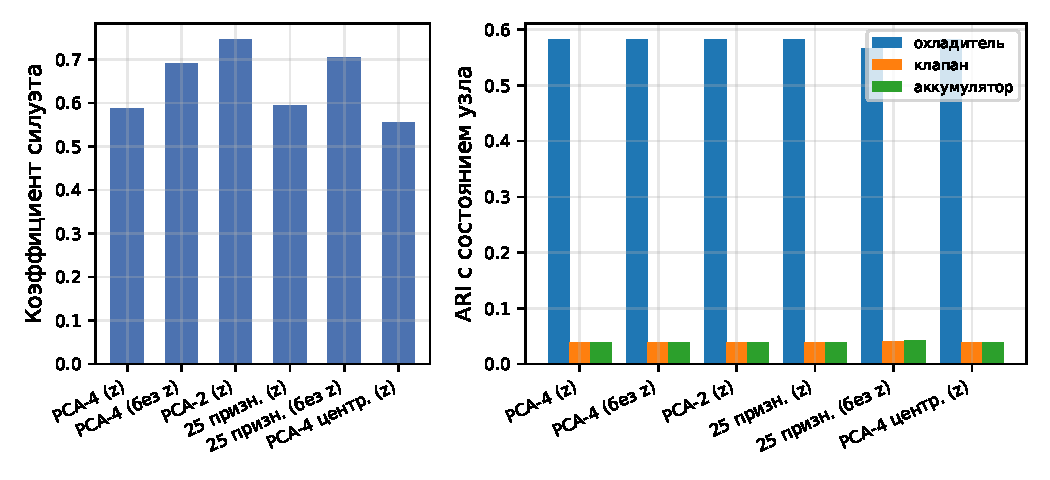
\includegraphics[width=\textwidth]{figures/fig14_sensitivity.pdf}
\caption{Силуэт и ARI с состояниями узлов при разных наборах координат и
масштабировании (KMeans, $k=3$)}
\label{fig:sens}
\end{figure}

\begin{table}[H]
\centering
\small
\caption{Чувствительность KMeans ($k = 3$) к выбору координат и масштабированию}\label{tab:sensitivity}
\begin{tabular}{lrrrr}
\toprule
Вариант координат & Силуэт & ARI охл. & ARI клап. & ARI акк. \\
\midrule
PCA-4 (z) & 0,588 & 0,582 & 0,038 & 0,039 \\
PCA-4 (без z) & 0,691 & 0,582 & 0,038 & 0,039 \\
PCA-2 (z) & 0,745 & 0,582 & 0,038 & 0,039 \\
25 призн. (z) & 0,594 & 0,582 & 0,038 & 0,039 \\
25 призн. (без z) & 0,706 & 0,565 & 0,040 & 0,043 \\
PCA-4 центр. (z) & 0,554 & 0,582 & 0,038 & 0,039 \\
\bottomrule
\end{tabular}
\end{table}


% ============================================================================
\section{ОБСУЖДЕНИЕ: ЧТО ОБНАРУЖЕНО, ЧТО АРТЕФАКТ, ЧТО УТВЕРЖДАТЬ НЕЛЬЗЯ}
% ============================================================================

\subsection{Что реально обнаружено}

\begin{enumerate}
\item \textbf{Главная ось смешанная.} Первая компонента стандартизованного
  PCA и первый фактор FA связаны с температурой, вибрацией и мощностью
  одновременно; первый фактор FA при этом почти чистый температурный. Счёт
  по первой компоненте сильно коррелирует с номером цикла
  (\DriftPcOneCorr). Значит, данные содержат сильный нестационарный тренд,
  который нельзя приписать только состоянию охладителя.
\item \textbf{Три крупных режима.} Все три алгоритма выделяют ранний,
  средний и поздний блоки, совпадающие с блоками замены охладителя. Разбиение
  устойчиво (\KmStab{} у KMeans, \WardStab{} у Уорда).
\item \textbf{Внутри раннего блока есть подобласть.} \DataHighPressN{} циклов
  с повышенным давлением и пониженным расходом (циклы \DataHighPressRange)
  образуют отдельную группу (\KmSizeOne{} в подвыборке). Это же множество
  помечено как «выбросы» по правилу 1,5 IQR, то есть правило указывает на
  реальный режим, а не на ошибки.
\item \textbf{Переходный режим.} DBSCAN отделяет от раннего блока группу из
  \DbSizeOne{} циклов, в которой \DbStableOne~\% составляют неустановившиеся
  режимы. KMeans и Уорд этого различия не делают.
\item \textbf{Клапан, насос и гидроаккумулятор не кластеризуются.} ARI не выше
  \KmAriPump, доли уровней клапана одинаковы по третям. Это отрицательный
  результат, но он устойчив.
\end{enumerate}

\subsection{Что является артефактом}

\begin{enumerate}
\item \textbf{«Почти двумерность» центрированной PCA.} Накопленная доля двух
  компонент \PcaCentCumTwo~--- следствие того, что мощность в ваттах имеет
  несопоставимо большой разброс. После стандартизации две компоненты дают
  лишь \PcaCumTwo.
\item \textbf{Рост силуэта при $k \ge 5$.} Он вызван группами из
  \KFiveSizeMin{} и \KSixSizeMin{} объектов; правило минимального размера
  группы отсекает такие решения.
\item \textbf{Высокий силуэт без $z$-масштабирования.} Значения
  \SensSilPcFourRaw{} и \SensSilPcTwoZ{} не означают лучшего разбиения:
  ARI с метками при этом не меняется. Силуэт чувствителен к масштабу и
  размерности, поэтому сравнивать его между пространствами нельзя.
\item \textbf{Высокий ARI с охладителем.} Он частично объясняется тем, что
  метка меняется блоками, совпадающими по времени с третями кампании.
  Диагностической ценности сам по себе он не имеет.
\item \textbf{Силуэт DBSCAN.} Он посчитан без \DbNoise~\% точек шума, поэтому
  слегка завышен по сравнению с KMeans, где шума нет.
\item \textbf{Нумерация групп.} Она произвольна у всех алгоритмов; в отчёте
  группы упорядочены по медианному номеру цикла, и это удобство, а не
  свойство данных.
\end{enumerate}

\subsection{Что утверждать нельзя}

\begin{enumerate}
\item \textbf{Нельзя диагностировать клапан, насос и гидроаккумулятор} по
  найденным группам: их состояния не образуют отдельных областей, ARI близок
  к нулю.
\item \textbf{Нельзя переносить кластеры Уорда и DBSCAN на новые циклы.} У
  Уорда нет метода предсказания, у DBSCAN новые точки могут оказаться шумом.
  У KMeans метод \texttt{predict} есть, но результат зависит от масштаба
  координат и от PCA, обученной на старой части кампании.
\item \textbf{Нельзя утверждать, что режимов ровно три.} Число групп выбрано
  по объявленному правилу; при другой допустимой погрешности силуэта
  разумным был бы и $k=4$.
\item \textbf{Нельзя приписывать падение температуры только деградации
  охладителя.} Температура, вибрация и мощность меняются вместе с номером
  цикла; причинный вывод требует управления режимом, которого в наблюдениях
  нет.
\item \textbf{Нельзя переносить выводы за пределы этого стенда и этой
  кампании.} Набор получен на одном оборудовании при фиксированной программе
  испытаний.
\end{enumerate}

% ============================================================================
\struct{ЗАКЛЮЧЕНИЕ}
% ============================================================================

\noindent
В работе выполнены снижение размерности и кластеризация \DataCycles{} циклов
гидравлического испытательного стенда. Из \DataFeaturesAll{} циклопризнаков в
анализ включены \DataFeaturesUsed{}; постоянные и почти постоянные признаки
исключены после аудита.

Ответ на вопрос В1 отрицательный: главная ось вариации не является чисто
тепловой. Она смешивает тепловое состояние охладительной линии и медленный
дрейф кампании (температура падает с \DriftTsOneEarly{} до \DriftTsOneLate~°C,
корреляция первой компоненты с номером цикла \DriftPcOneCorr). Факторный
анализ даёт более чистые оси: первый фактор почти совпадает с температурой,
второй~--- с мощностью и давлением.

Ответ на вопрос В2 также отрицательный для клапана, насоса и
гидроаккумулятора: их состояния не образуют отдельных групп (ARI не выше
\KmAriPump), а доли уровней клапана одинаковы по третям кампании. Единственная
устойчивая структура~--- деление на блоки, совпадающие с заменой охладителя,
плюс подобласть повышенного давления в раннем блоке и переходный
неустановившийся участок, который отделяет DBSCAN.

Практический итог: для сжатия данных следует использовать стандартизованную
PCA (четыре компоненты дают \ClustSharePct~\% дисперсии), для интерпретации
осей~--- факторный анализ, а для кластеризации~--- KMeans или Уорд с проверкой
устойчивости; DBSCAN полезен как индикатор переходных режимов и шума.
Полученная структура пригодна для описания режимов стенда, но не для
диагностики клапана, насоса и гидроаккумулятора и не для причинных выводов о
деградации оборудования.

% ============================================================================
\struct{СПИСОК ИСПОЛЬЗОВАННЫХ ИСТОЧНИКОВ}

\begin{thebibliography}{11}

\bibitem{uci} Condition Monitoring of Hydraulic Systems [Электронный ресурс] //
UCI Machine Learning Repository. --- 2018. --- DOI 10.24432/C5CW21. ---
URL: \url{https://archive.ics.uci.edu/dataset/447} (дата обращения:
24.11.2026).

\bibitem{gost} ГОСТ 7.32-2017. Система стандартов по информации,
библиотечному и издательскому делу. Отчёт о научно-исследовательской работе.
Структура и правила оформления. --- М.: Стандартинформ, 2017. --- 32~с.

\bibitem{jolliffe} Jolliffe I.~T. Principal Component Analysis. --- 2nd ed. ---
New York: Springer, 2002. --- 487~p.

\bibitem{harman} Harman H.~H. Modern Factor Analysis. --- 3rd ed. ---
Chicago: University of Chicago Press, 1976. --- 487~p.

\bibitem{macqueen} MacQueen J. Some methods for classification and analysis of
multivariate observations // Proceedings of the Fifth Berkeley Symposium on
Mathematical Statistics and Probability. --- 1967. --- Vol.~1. --- P.~281--297.

\bibitem{ward} Ward J.~H. Hierarchical grouping to optimize an objective
function // Journal of the American Statistical Association. --- 1963. ---
Vol.~58, no.~301. --- P.~236--244.

\bibitem{ester} Ester M., Kriegel H.-P., Sander J., Xu X. A density-based
algorithm for discovering clusters in large spatial databases with noise //
Proceedings of the Second International Conference on Knowledge Discovery and
Data Mining. --- 1996. --- P.~226--231.

\bibitem{rousseeuw} Rousseeuw P.~J. Silhouettes: a graphical aid to the
interpretation and validation of cluster analysis // Journal of Computational
and Applied Mathematics. --- 1987. --- Vol.~20. --- P.~53--65.

\bibitem{davies} Davies D.~L., Bouldin D.~W. A cluster separation measure //
IEEE Transactions on Pattern Analysis and Machine Intelligence. --- 1979. ---
Vol.~PAMI-1, no.~2. --- P.~224--227.

\bibitem{hubert} Hubert L., Arabie P. Comparing partitions // Journal of
Classification. --- 1985. --- Vol.~2, no.~1. --- P.~193--218.

\bibitem{sklearn} Pedregosa F., Varoquaux G., Gramfort A. et al. Scikit-learn:
machine learning in Python // Journal of Machine Learning Research. ---
2011. --- Vol.~12. --- P.~2825--2830.

\end{thebibliography}

% ============================================================================
\struct{ПРИЛОЖЕНИЕ А. МАТРИЦЫ СОПРЯЖЁННОСТИ}
% ============================================================================

\noindent
Таблица~\ref{tab:crosstab} показывает, как группы KMeans распределены по
уровням состояний узлов. По охладителю группы почти чистые, по клапану и
гидроаккумулятору уровни перемешаны.

\begin{table}[H]
\centering
\small
\caption{Матрицы сопряжённости групп KMeans и состояний узлов (число циклов подвыборки)}\label{tab:crosstab}
\begin{center}\textit{Охладитель, \%}\end{center}
\begin{tabular}{lrrrr}
\toprule
Группа & 3 & 20 & 100 & Всего \\
\midrule
1 & 127 & 0 & 0 & 127 \\
2 & 266 & 407 & 2 & 675 \\
3 & 0 & 0 & 398 & 398 \\
\bottomrule
\end{tabular}
\par\medskip
\begin{center}\textit{Клапан, \%}\end{center}
\begin{tabular}{lrrrrr}
\toprule
Группа & 73 & 80 & 90 & 100 & Всего \\
\midrule
1 & 32 & 29 & 32 & 34 & 127 \\
2 & 104 & 104 & 95 & 372 & 675 \\
3 & 59 & 74 & 61 & 204 & 398 \\
\bottomrule
\end{tabular}
\par\medskip
\begin{center}\textit{Гидроаккумулятор, бар}\end{center}
\begin{tabular}{lrrrrr}
\toprule
Группа & 90 & 100 & 115 & 130 & Всего \\
\midrule
1 & 41 & 48 & 37 & 1 & 127 \\
2 & 234 & 97 & 95 & 249 & 675 \\
3 & 183 & 73 & 72 & 70 & 398 \\
\bottomrule
\end{tabular}
\end{table}


% ============================================================================
\struct{ПРИЛОЖЕНИЕ Б. ПРОФИЛИ ГРУПП}
% ============================================================================

\noindent
Таблица~\ref{tab:profile} содержит размер, положение во времени и состав по
охладителю для всех групп трёх алгоритмов.

\begin{table}[H]
\centering
\scriptsize
\caption{Профили итоговых групп: размер, положение во времени и состав по охладителю}\label{tab:profile}
\resizebox{\textwidth}{!}{%
\begin{tabular}{llrrrrrrr}
\toprule
Алгоритм & Группа & $n$ & Циклы & Медиана & Неустан., \% & Охл. 3, \% & Охл. 20, \% & Охл. 100, \% \\
\midrule
KMeans & 1 & 127 & 212--702 & 532 & 1,6 & 100,0 & 0,0 & 0,0 \\
KMeans & 2 & 675 & 8--1467 & 855 & 40,9 & 39,4 & 60,3 & 0,3 \\
KMeans & 3 & 398 & 1472--2205 & 1852 & 31,9 & 0,0 & 0,0 & 100,0 \\
\midrule
Ward & 1 & 118 & 212--691 & 521 & 0,8 & 100,0 & 0,0 & 0,0 \\
Ward & 2 & 684 & 8--1467 & 849 & 40,5 & 40,2 & 59,5 & 0,3 \\
Ward & 3 & 398 & 1472--2205 & 1852 & 31,9 & 0,0 & 0,0 & 100,0 \\
\midrule
DBSCAN & 1 & 224 & 25--732 & 235 & 50,4 & 100,0 & 0,0 & 0,0 \\
DBSCAN & 2 & 114 & 212--691 & 520 & 0,9 & 100,0 & 0,0 & 0,0 \\
DBSCAN & 3 & 405 & 740--1465 & 1104 & 34,3 & 0,0 & 99,8 & 0,2 \\
DBSCAN & 4 & 397 & 1472--2205 & 1853 & 32,0 & 0,0 & 0,0 & 100,0 \\
\bottomrule
\end{tabular}}
\end{table}


\end{document}
